\documentclass[12pt]{article}
\usepackage{graphicx}
\usepackage{placeins}
\title{Moodle Android App}
\author{Sai Deep (2012CS10223) \\ Mano Teja (2010CS50286) \\ TRK Saran (2010BB50042) }
\date{24 February 2016}
\begin{document}
\maketitle
\tableofcontents

\section{Introduction}
Our task was to design a frontend for the Moodle Android Application. We were provided with a locally deployable web2py server. We developed an android app which interacts with this server via API calls.
\section{User Interface}
\subsection{Primary Screen}
A layout with one field for entering username, one for entering password followed by a \textbf{Sign in} button. 
\begin{figure}[!ht]
	\centering
	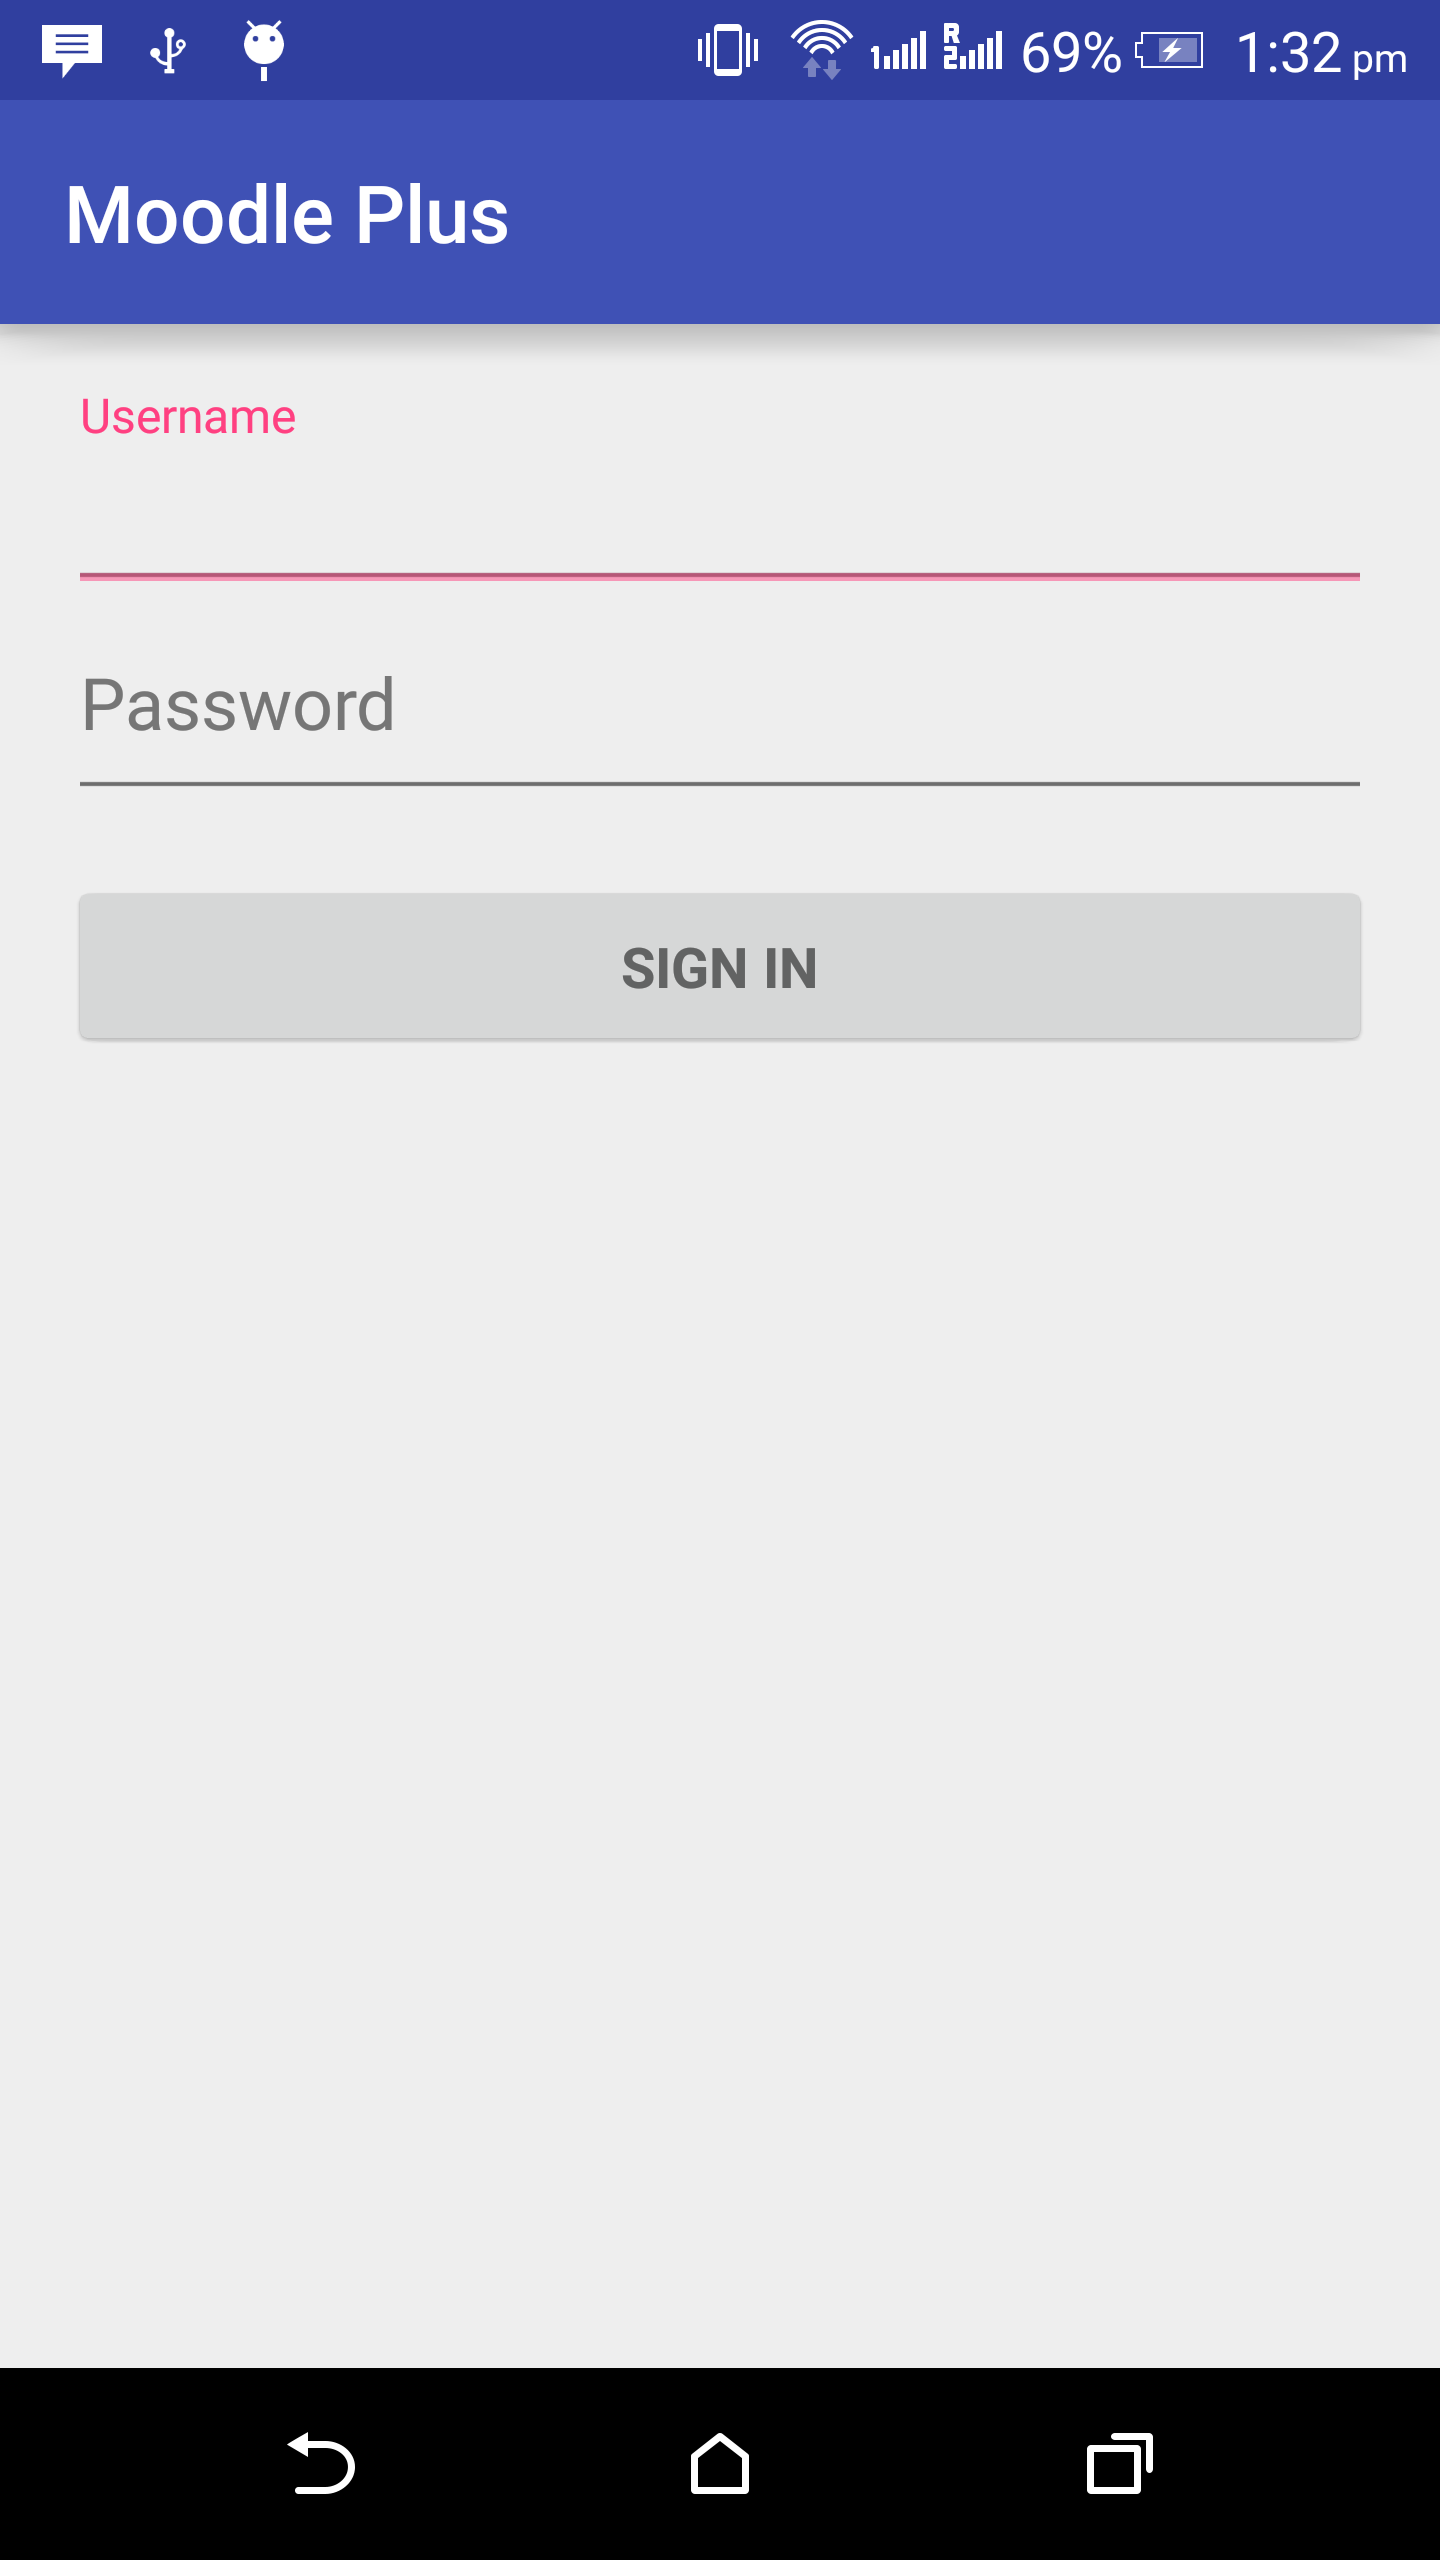
\includegraphics[width=0.4\textwidth]{images/login_screen.png}
	\caption{Primary Screen}
\end{figure}
\FloatBarrier
\subsubsection{Progress Bar}
A progress bar appears on clicking sign in  button when all the text inputs are non-empty and keeps spinning till response is received from server after which it disappears.

\subsection{Welcome Screen - After Logging in}
A list of registered courses are displayed.There are three buttons at the bottom of the screen for viewing notifications,grades and logging out.\\   
\begin{figure}[!ht]
	\centering
	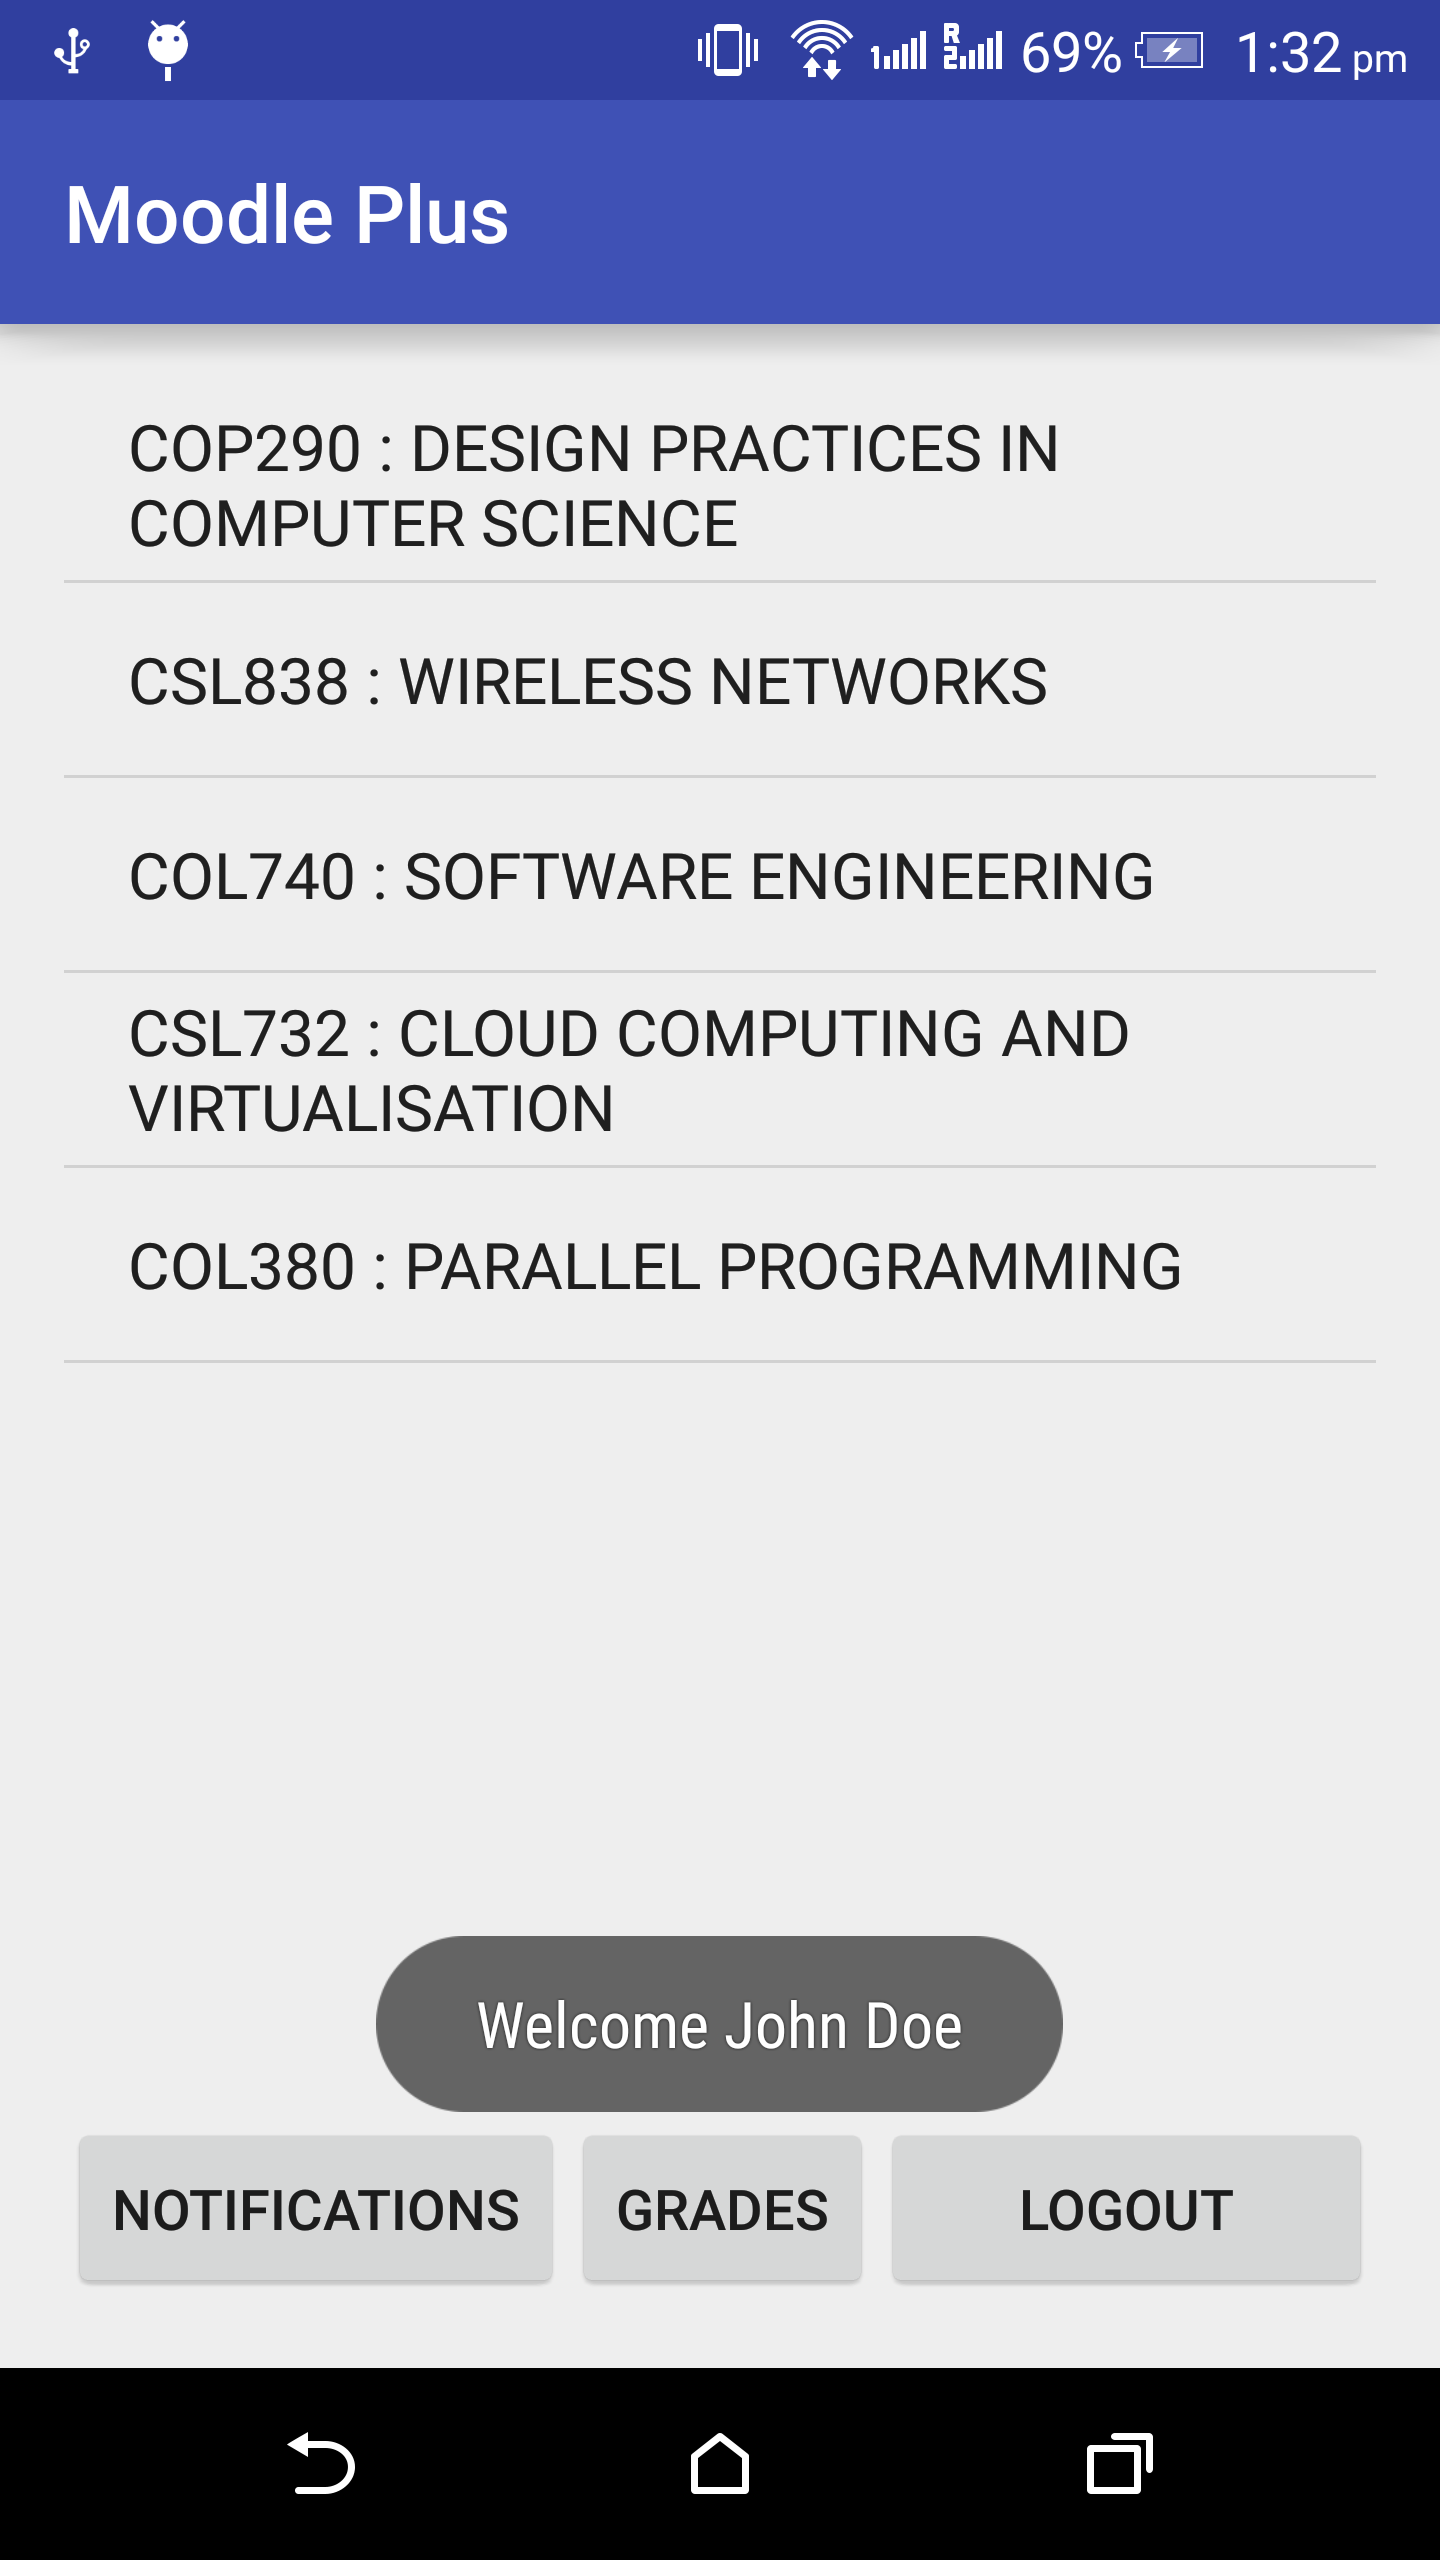
\includegraphics[width=0.4\textwidth]{images/Welcome_screen.png}
	\caption{Welcome Screen}
\end{figure}
\FloatBarrier

\subsection{On Clicking Notifications Button}
\begin{figure}[!ht]
	\centering
	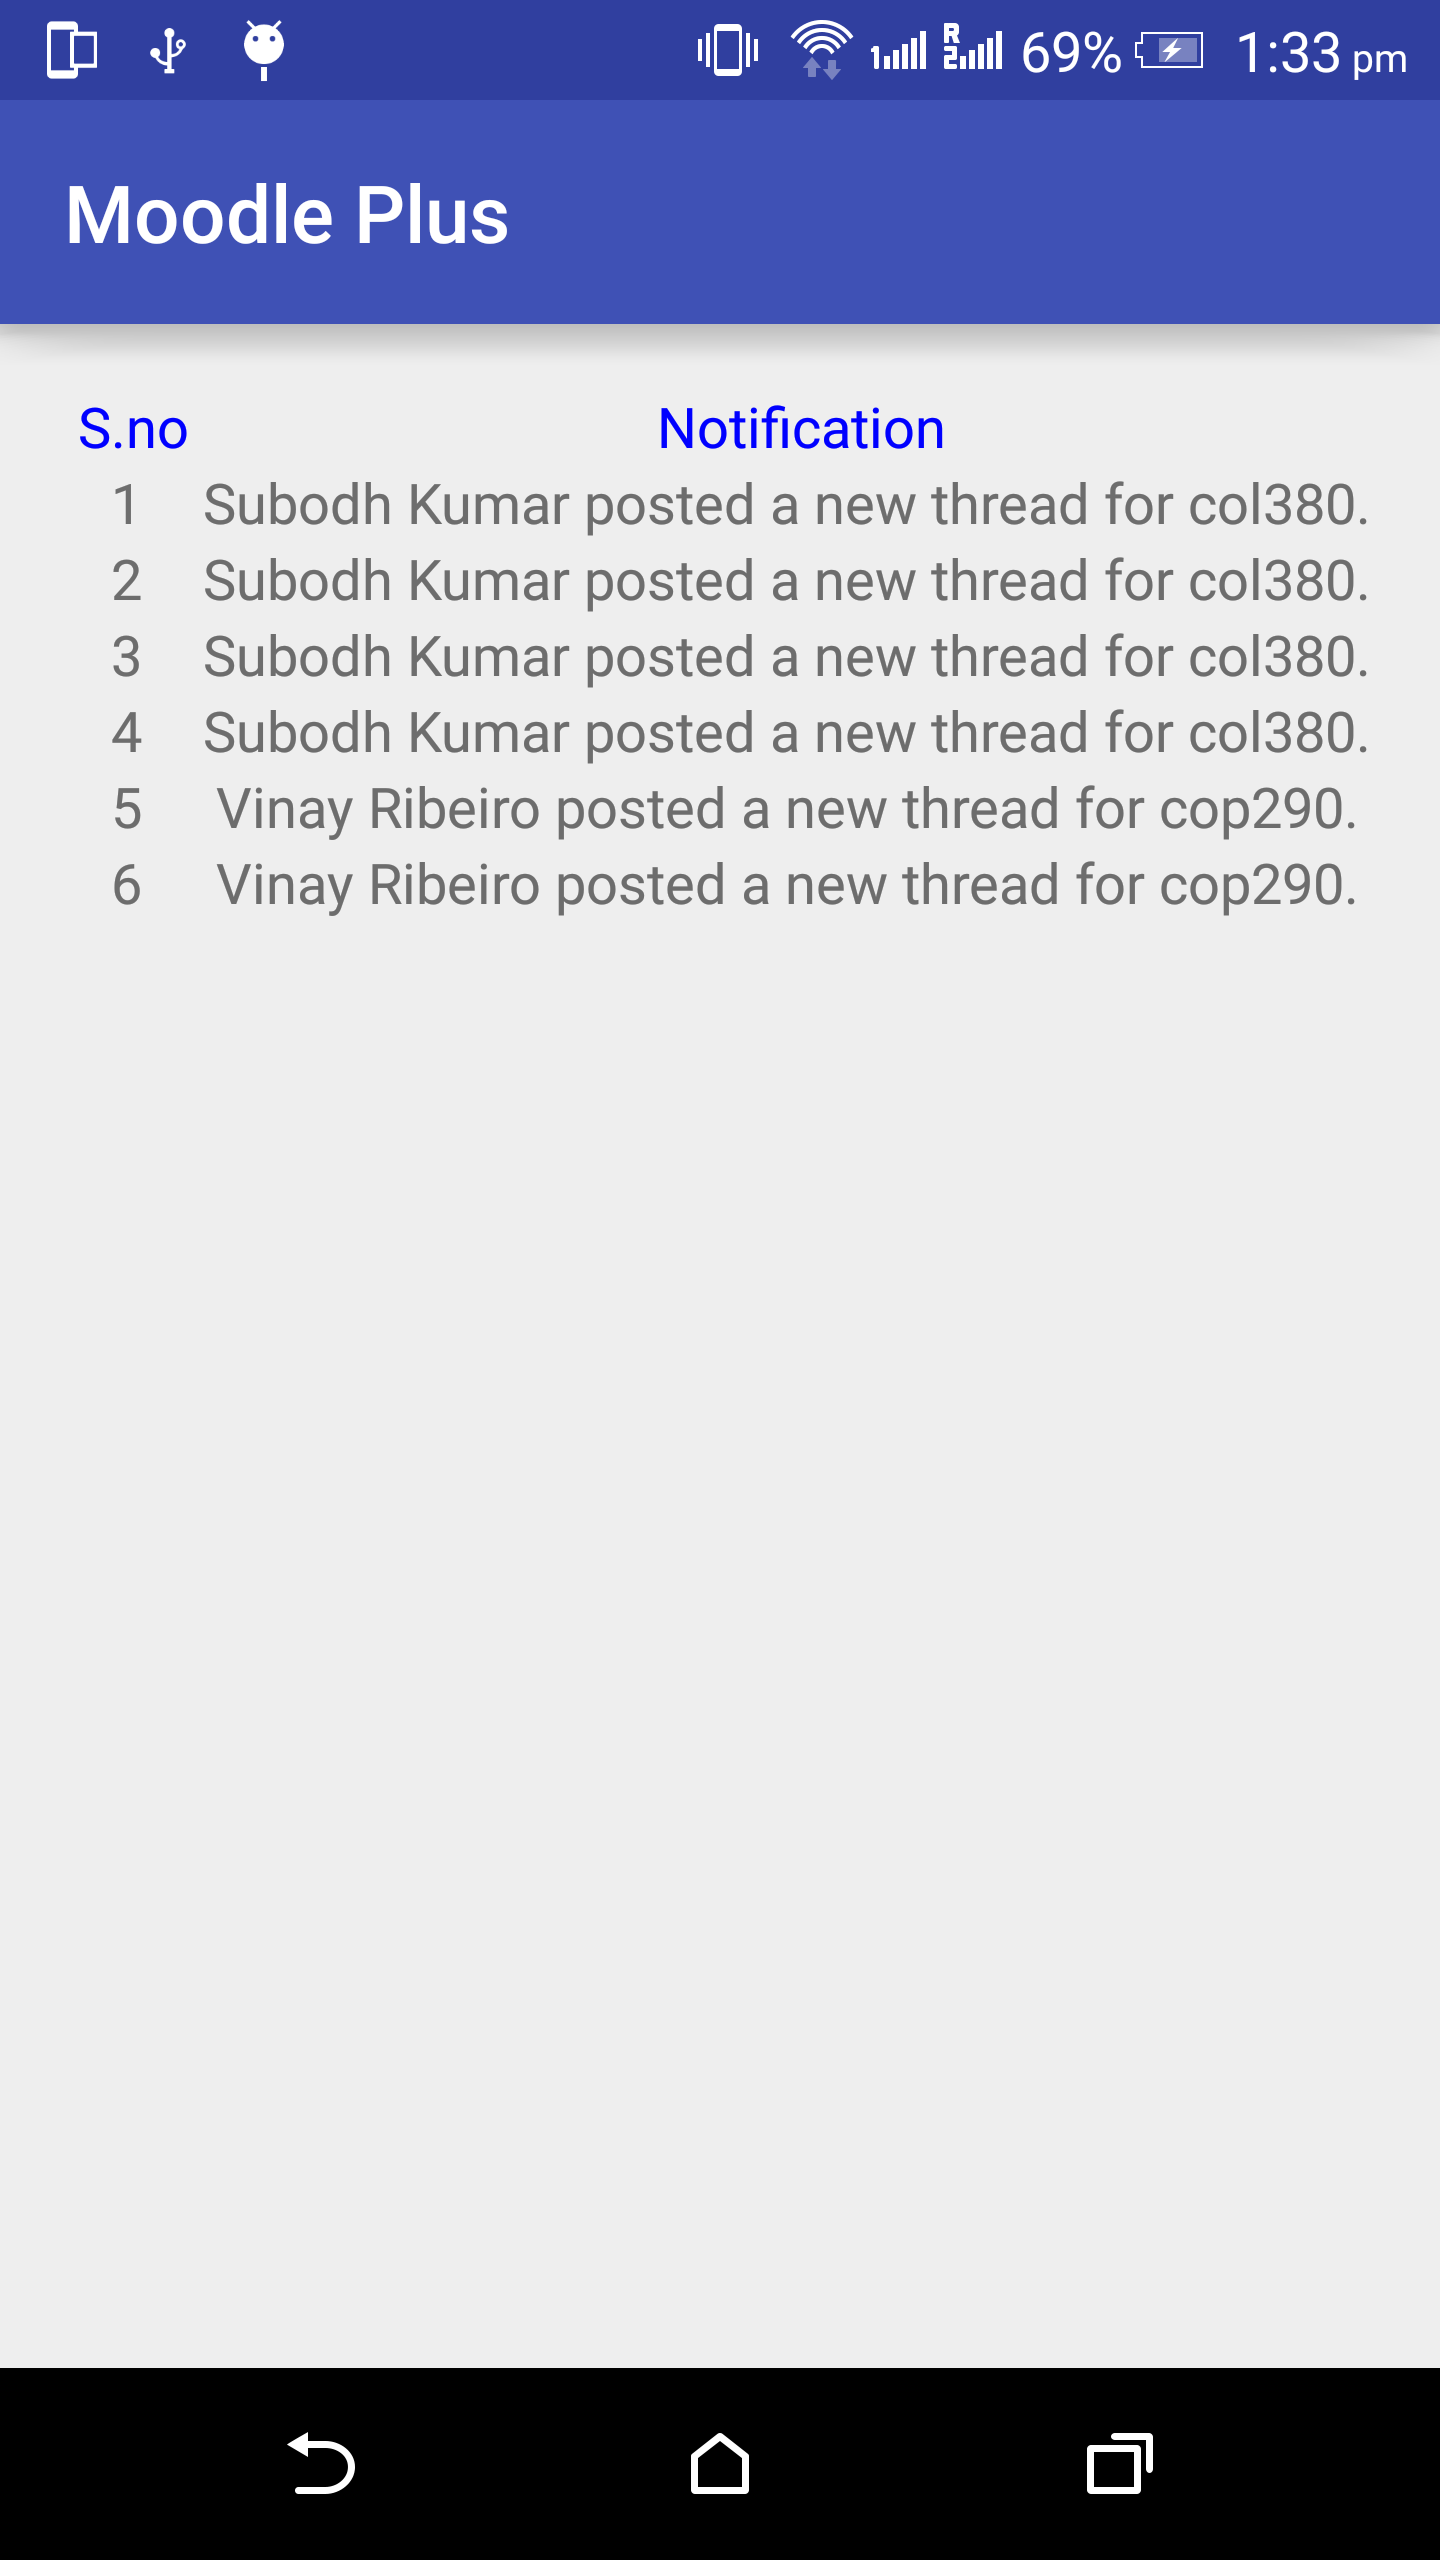
\includegraphics[width=0.4\textwidth]{images/notifications.png}
	\caption{Notifications Screen}
\end{figure}
\FloatBarrier
\subsection{On Clicking Grades Button}
\begin{figure}[!ht]
	\centering
	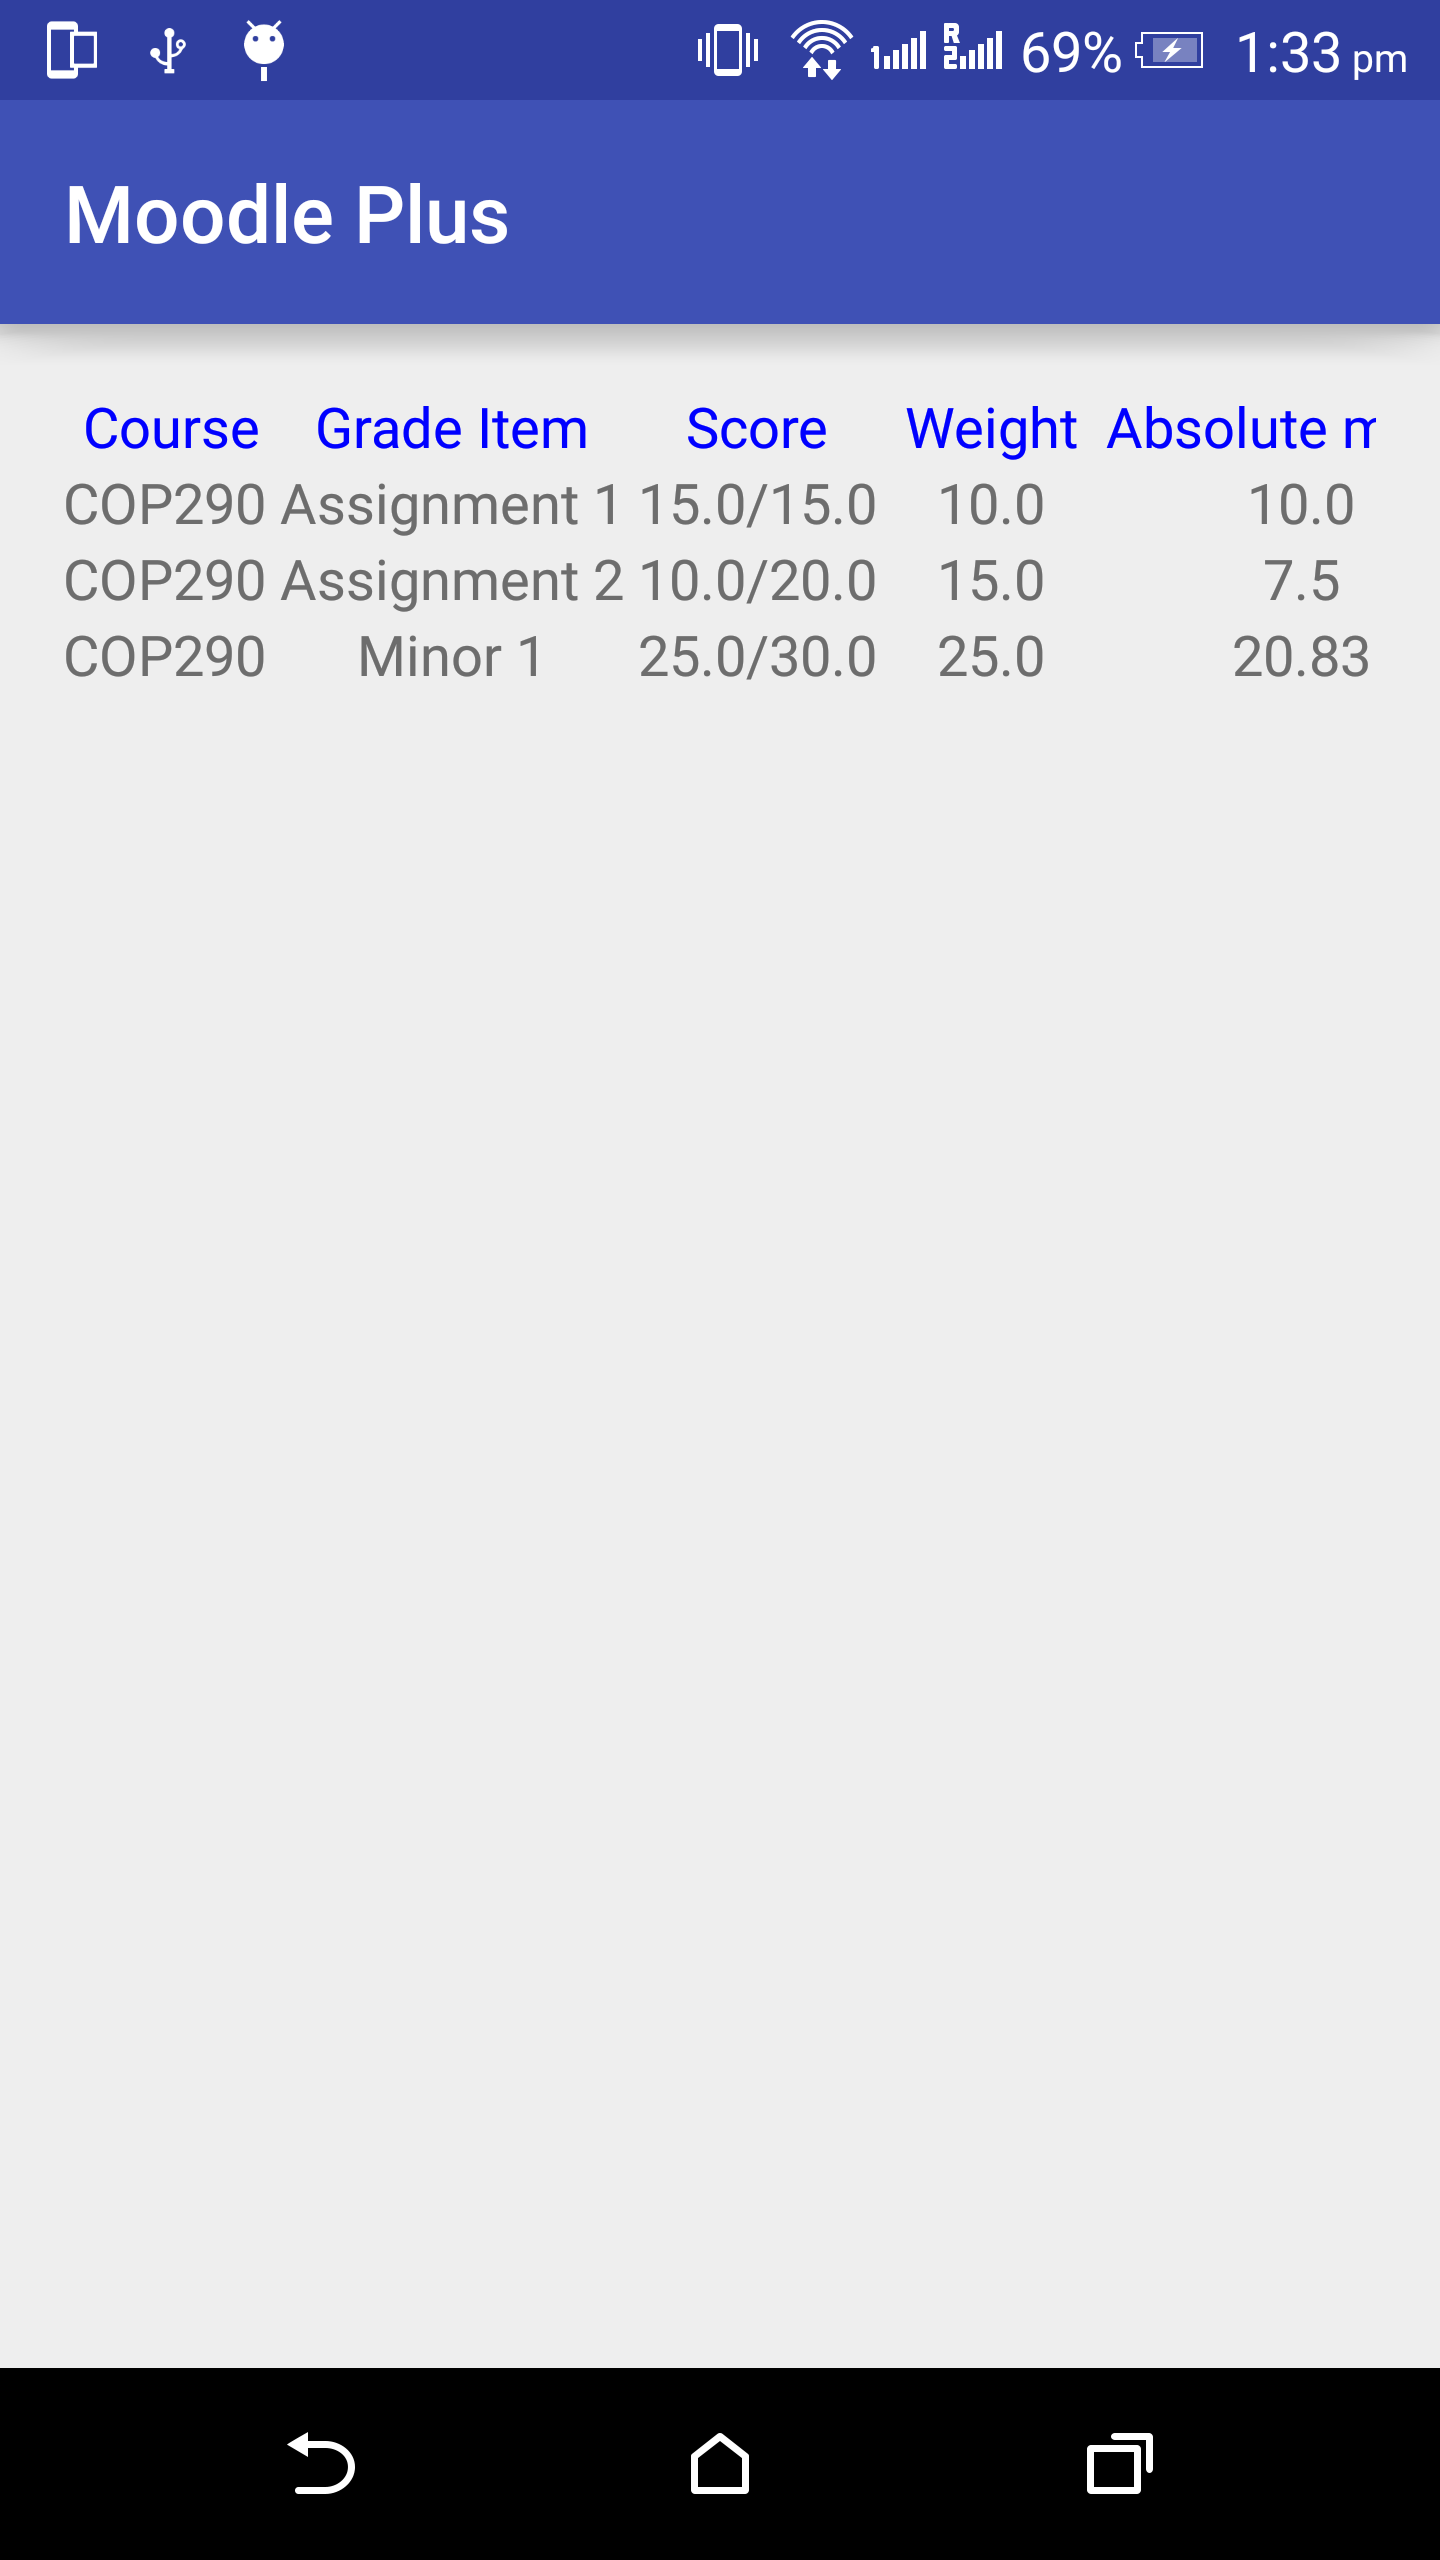
\includegraphics[width=0.4\textwidth]{images/allgrades.png}
	\caption{All Grades Screen}
\end{figure}
\FloatBarrier
\subsection{On Clicking Logout Button}
\begin{figure}[!ht]
	\centering
	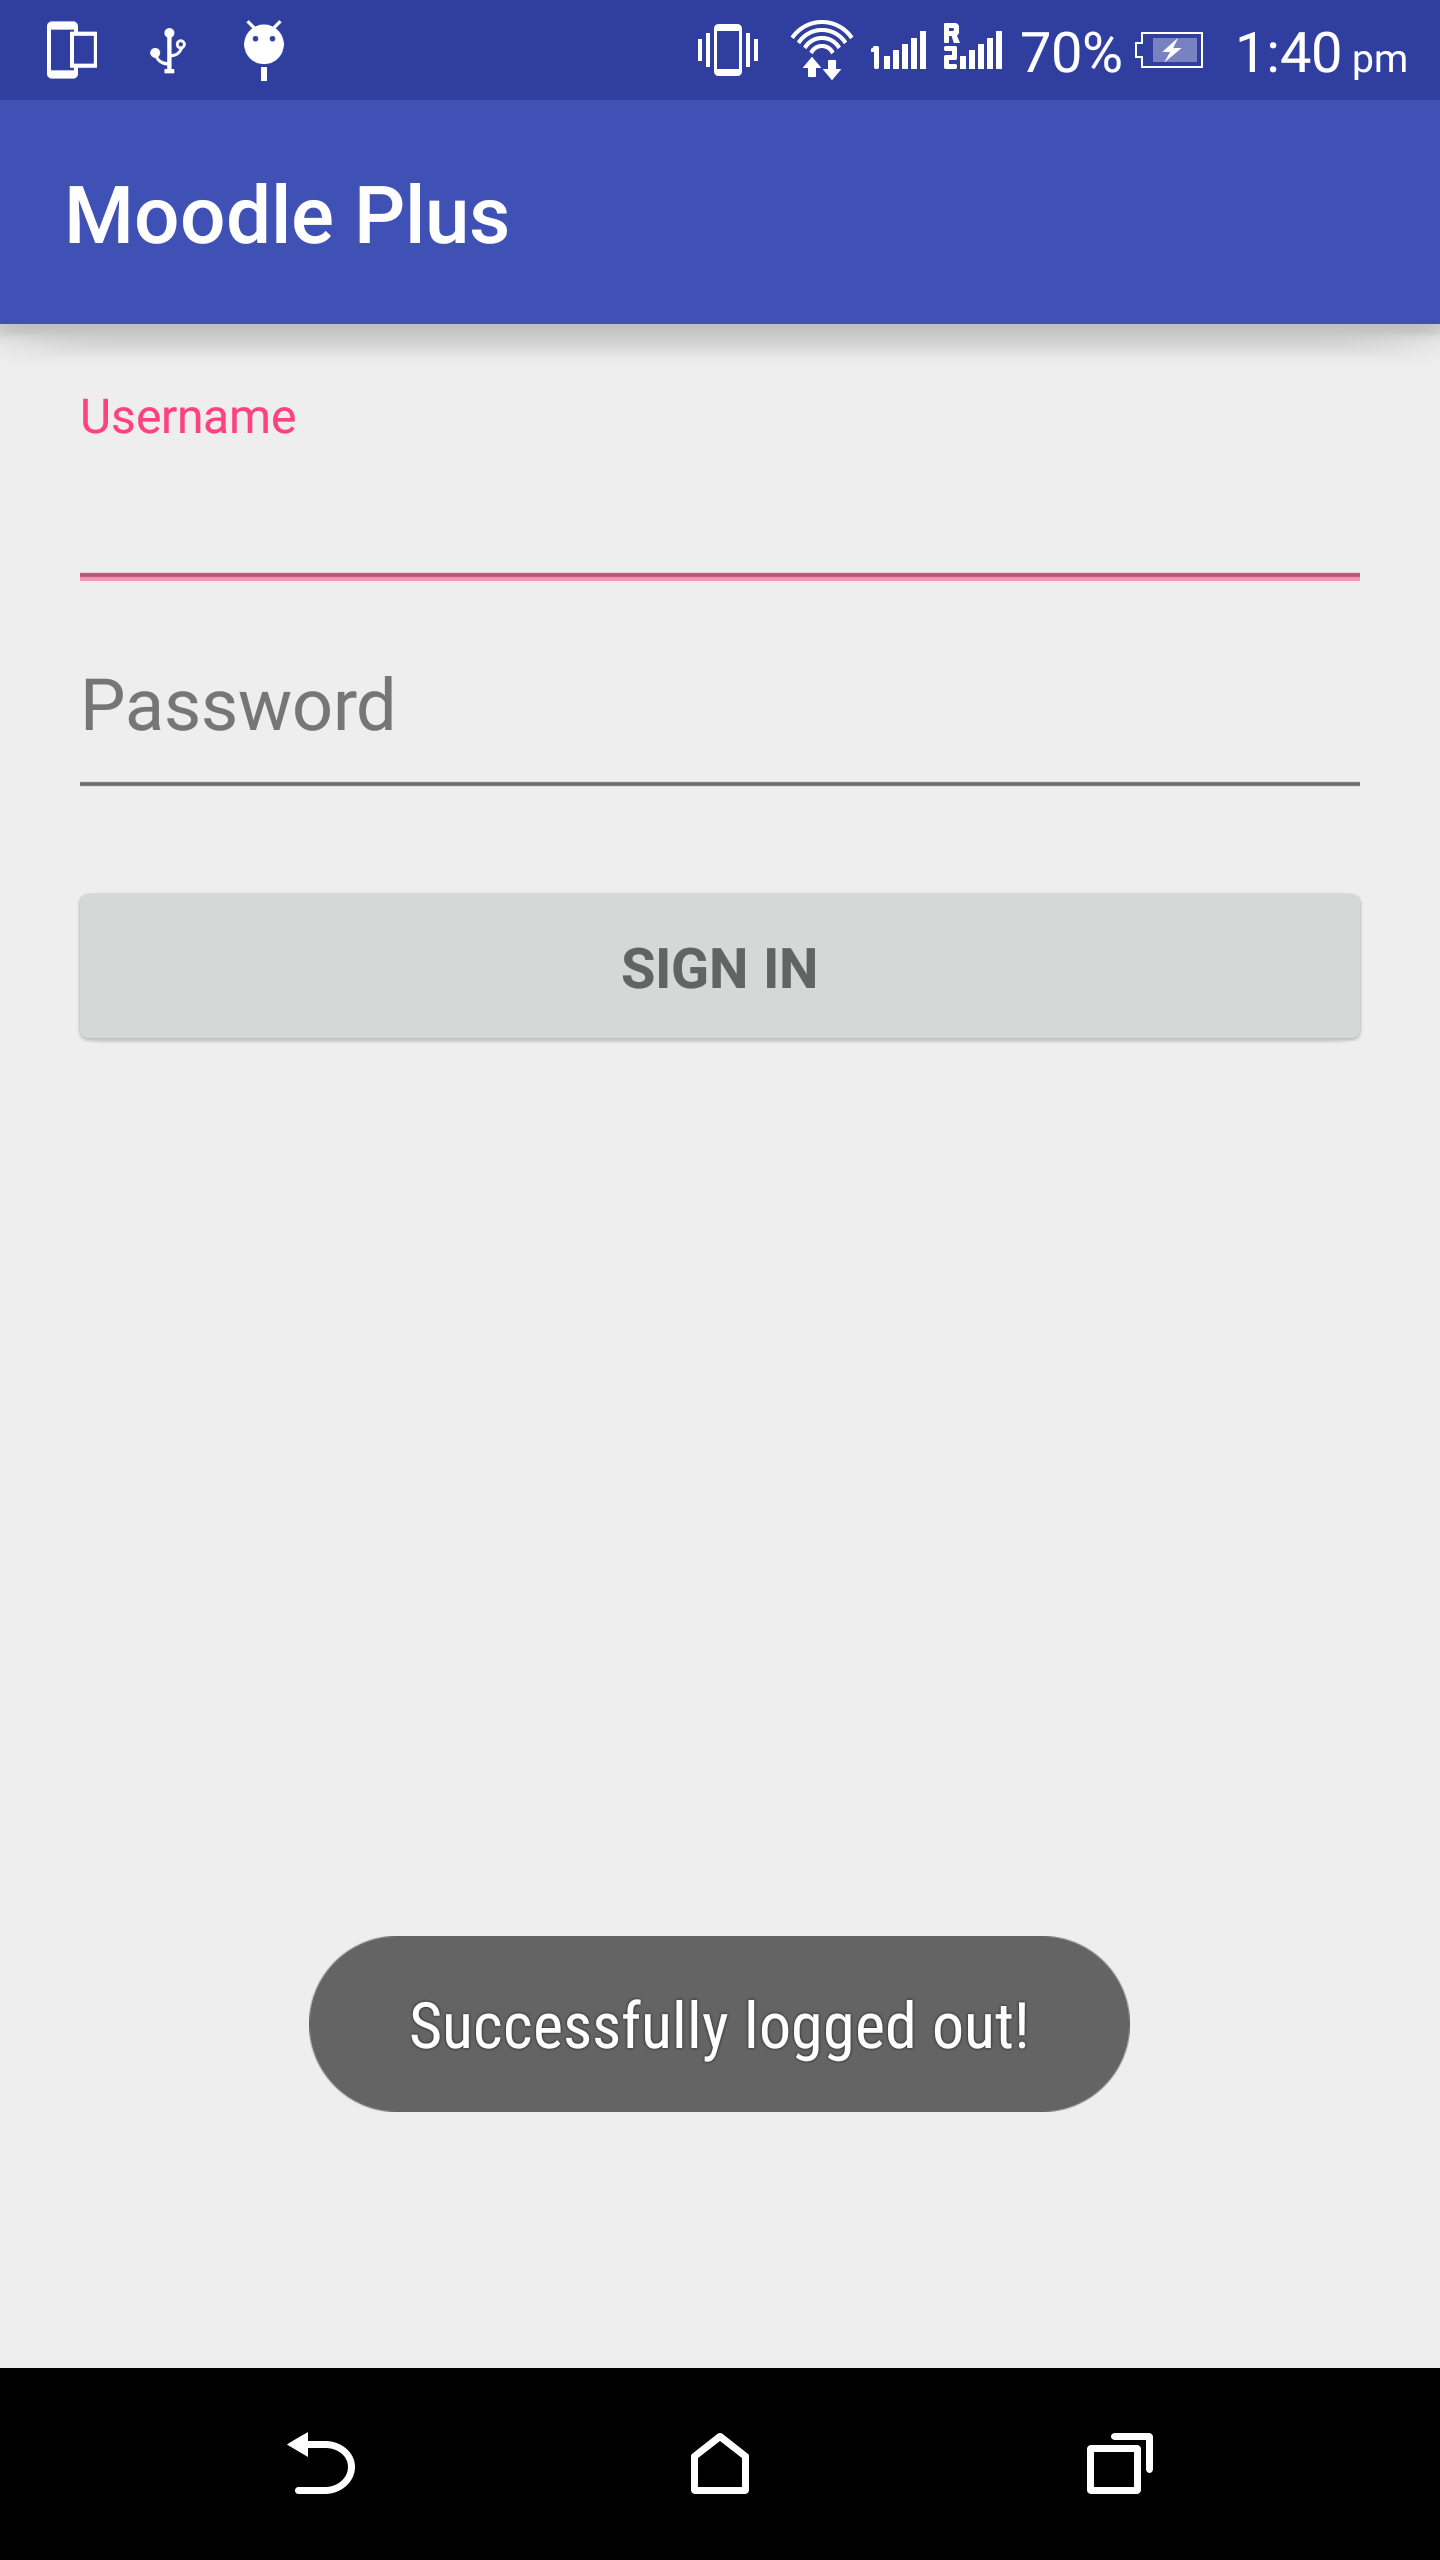
\includegraphics[width=0.4\textwidth]{images/logout.png}
	\caption{Successful Logout }
\end{figure}
\FloatBarrier
\subsection{Course Screen}
\subsubsection{After clicking on a particular course in home screen}
\begin{figure}[!ht]
	\centering
	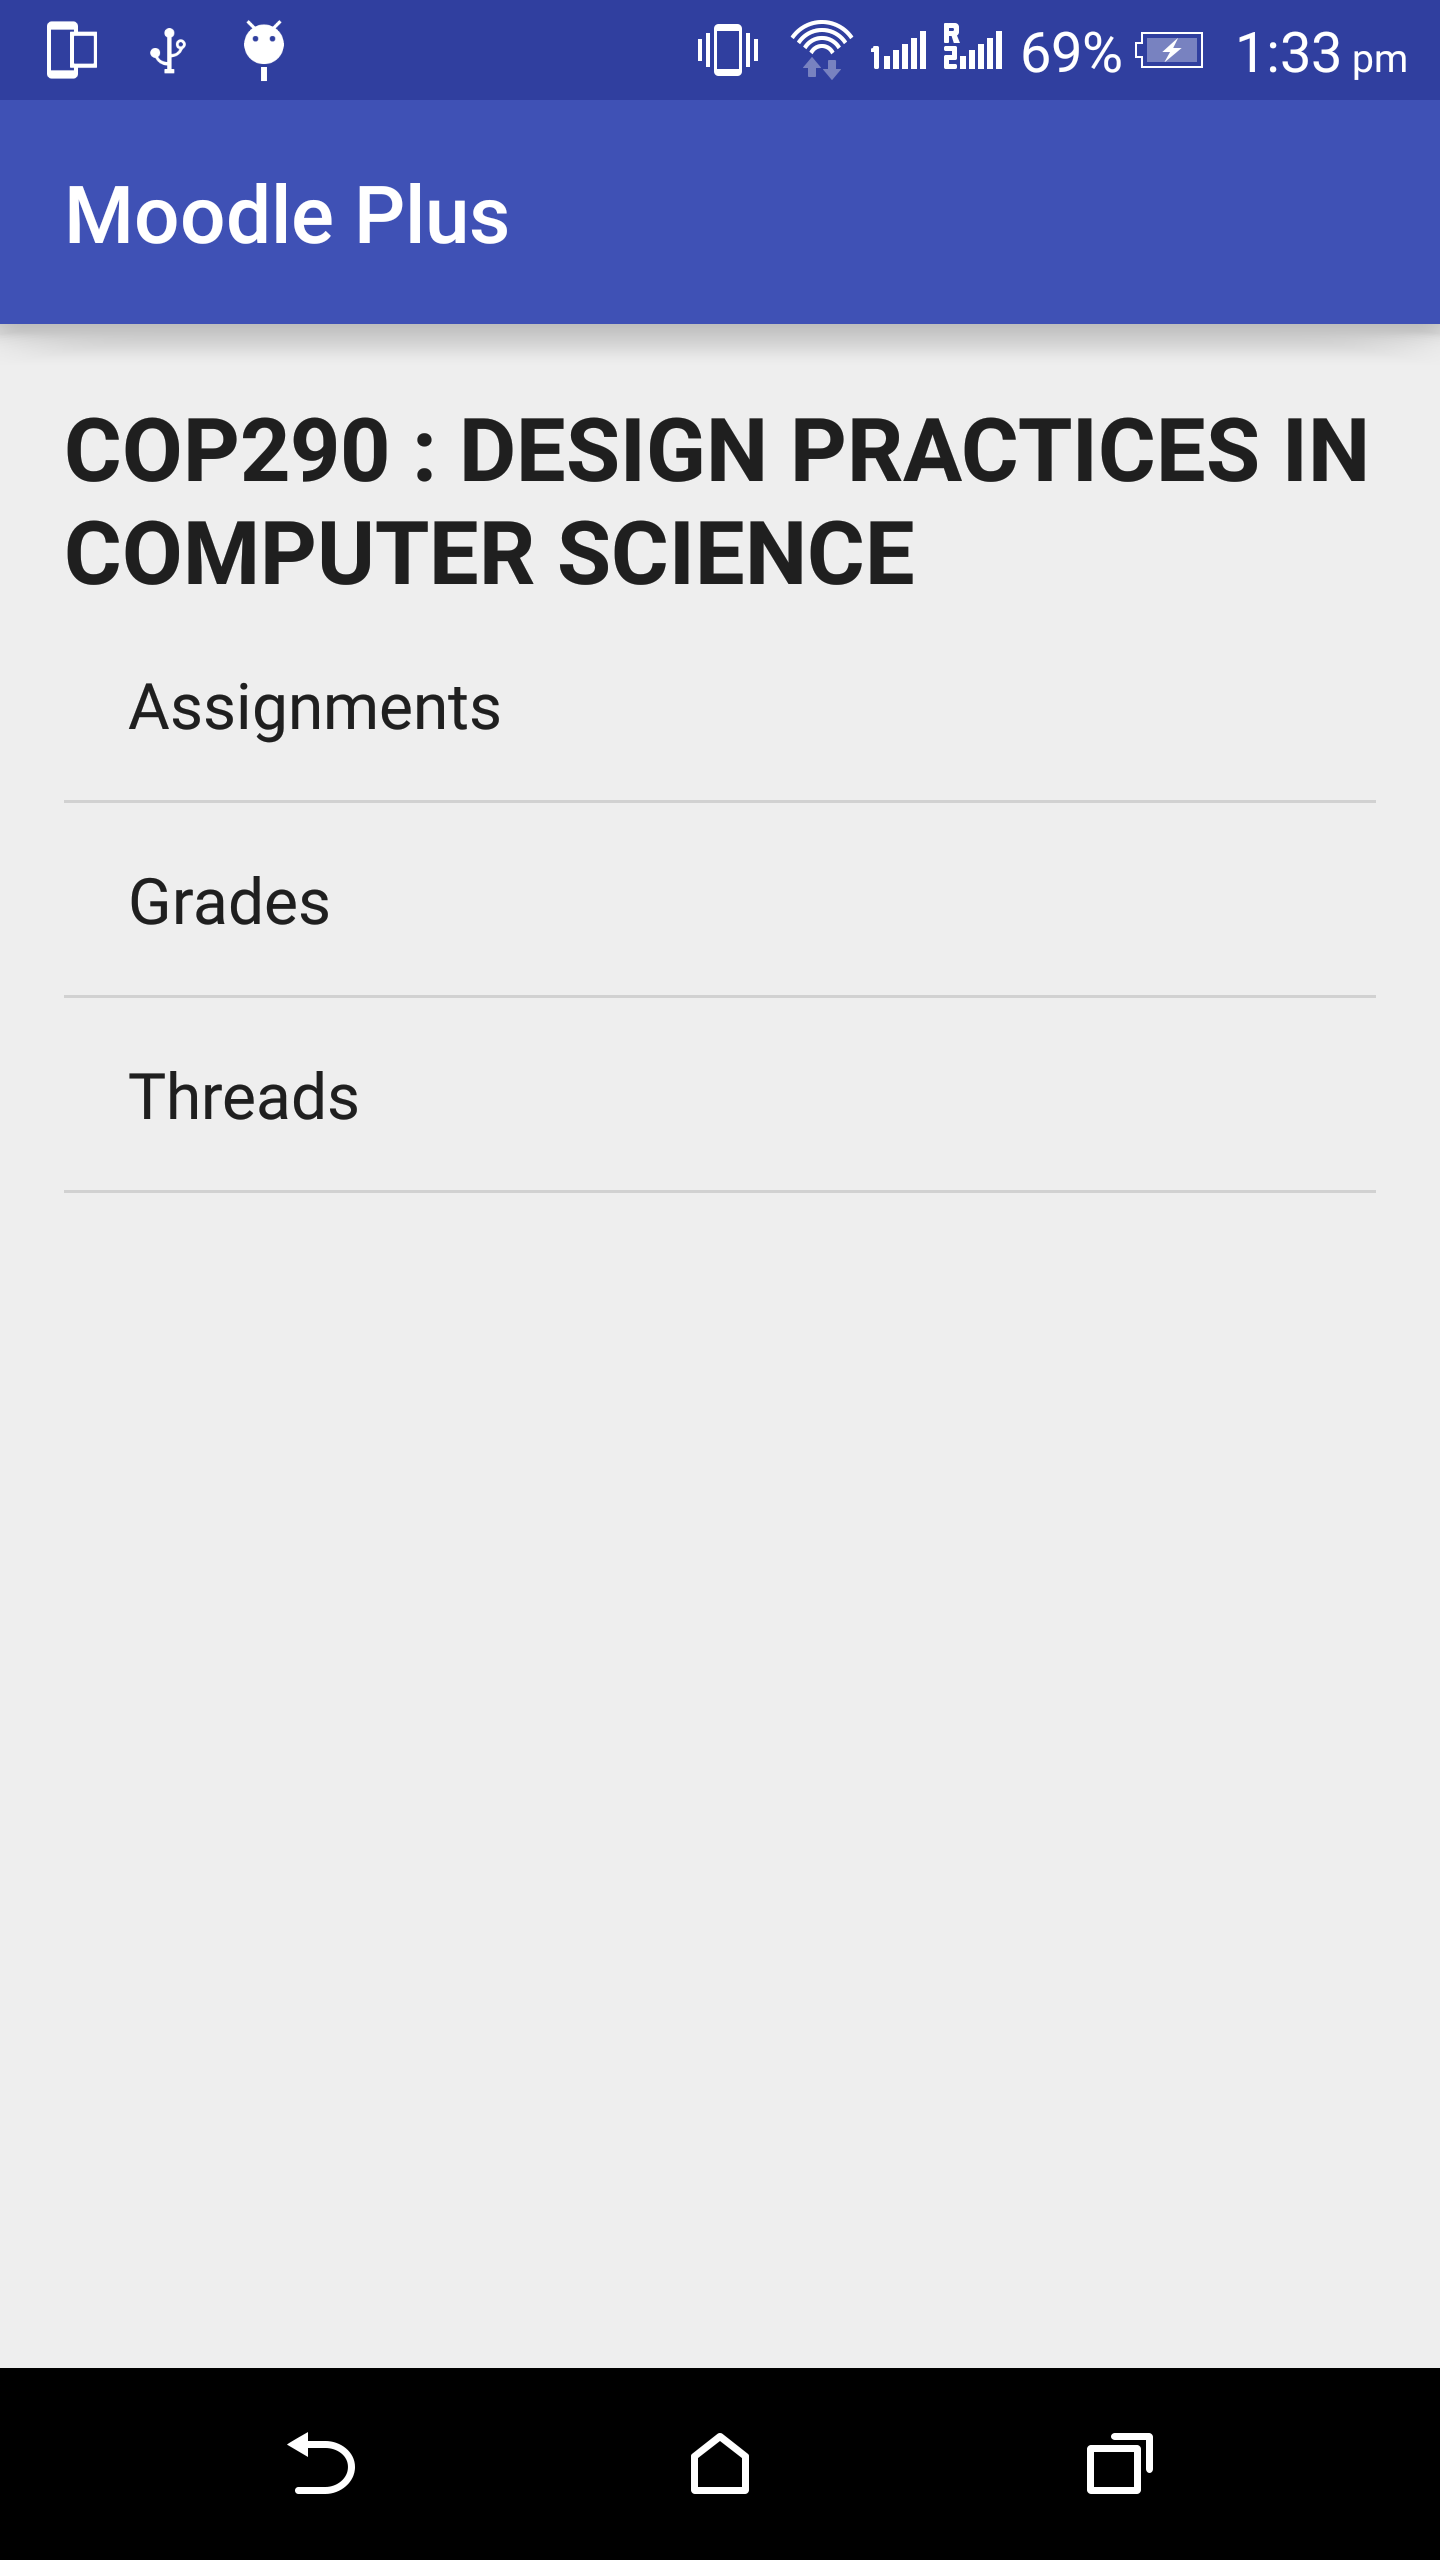
\includegraphics[width=0.4\textwidth]{images/course_contents.png}
	\caption{Course Screen}
\end{figure}
\FloatBarrier
\subsubsection{List of Assignments}
\begin{figure}[!ht]
	\centering
	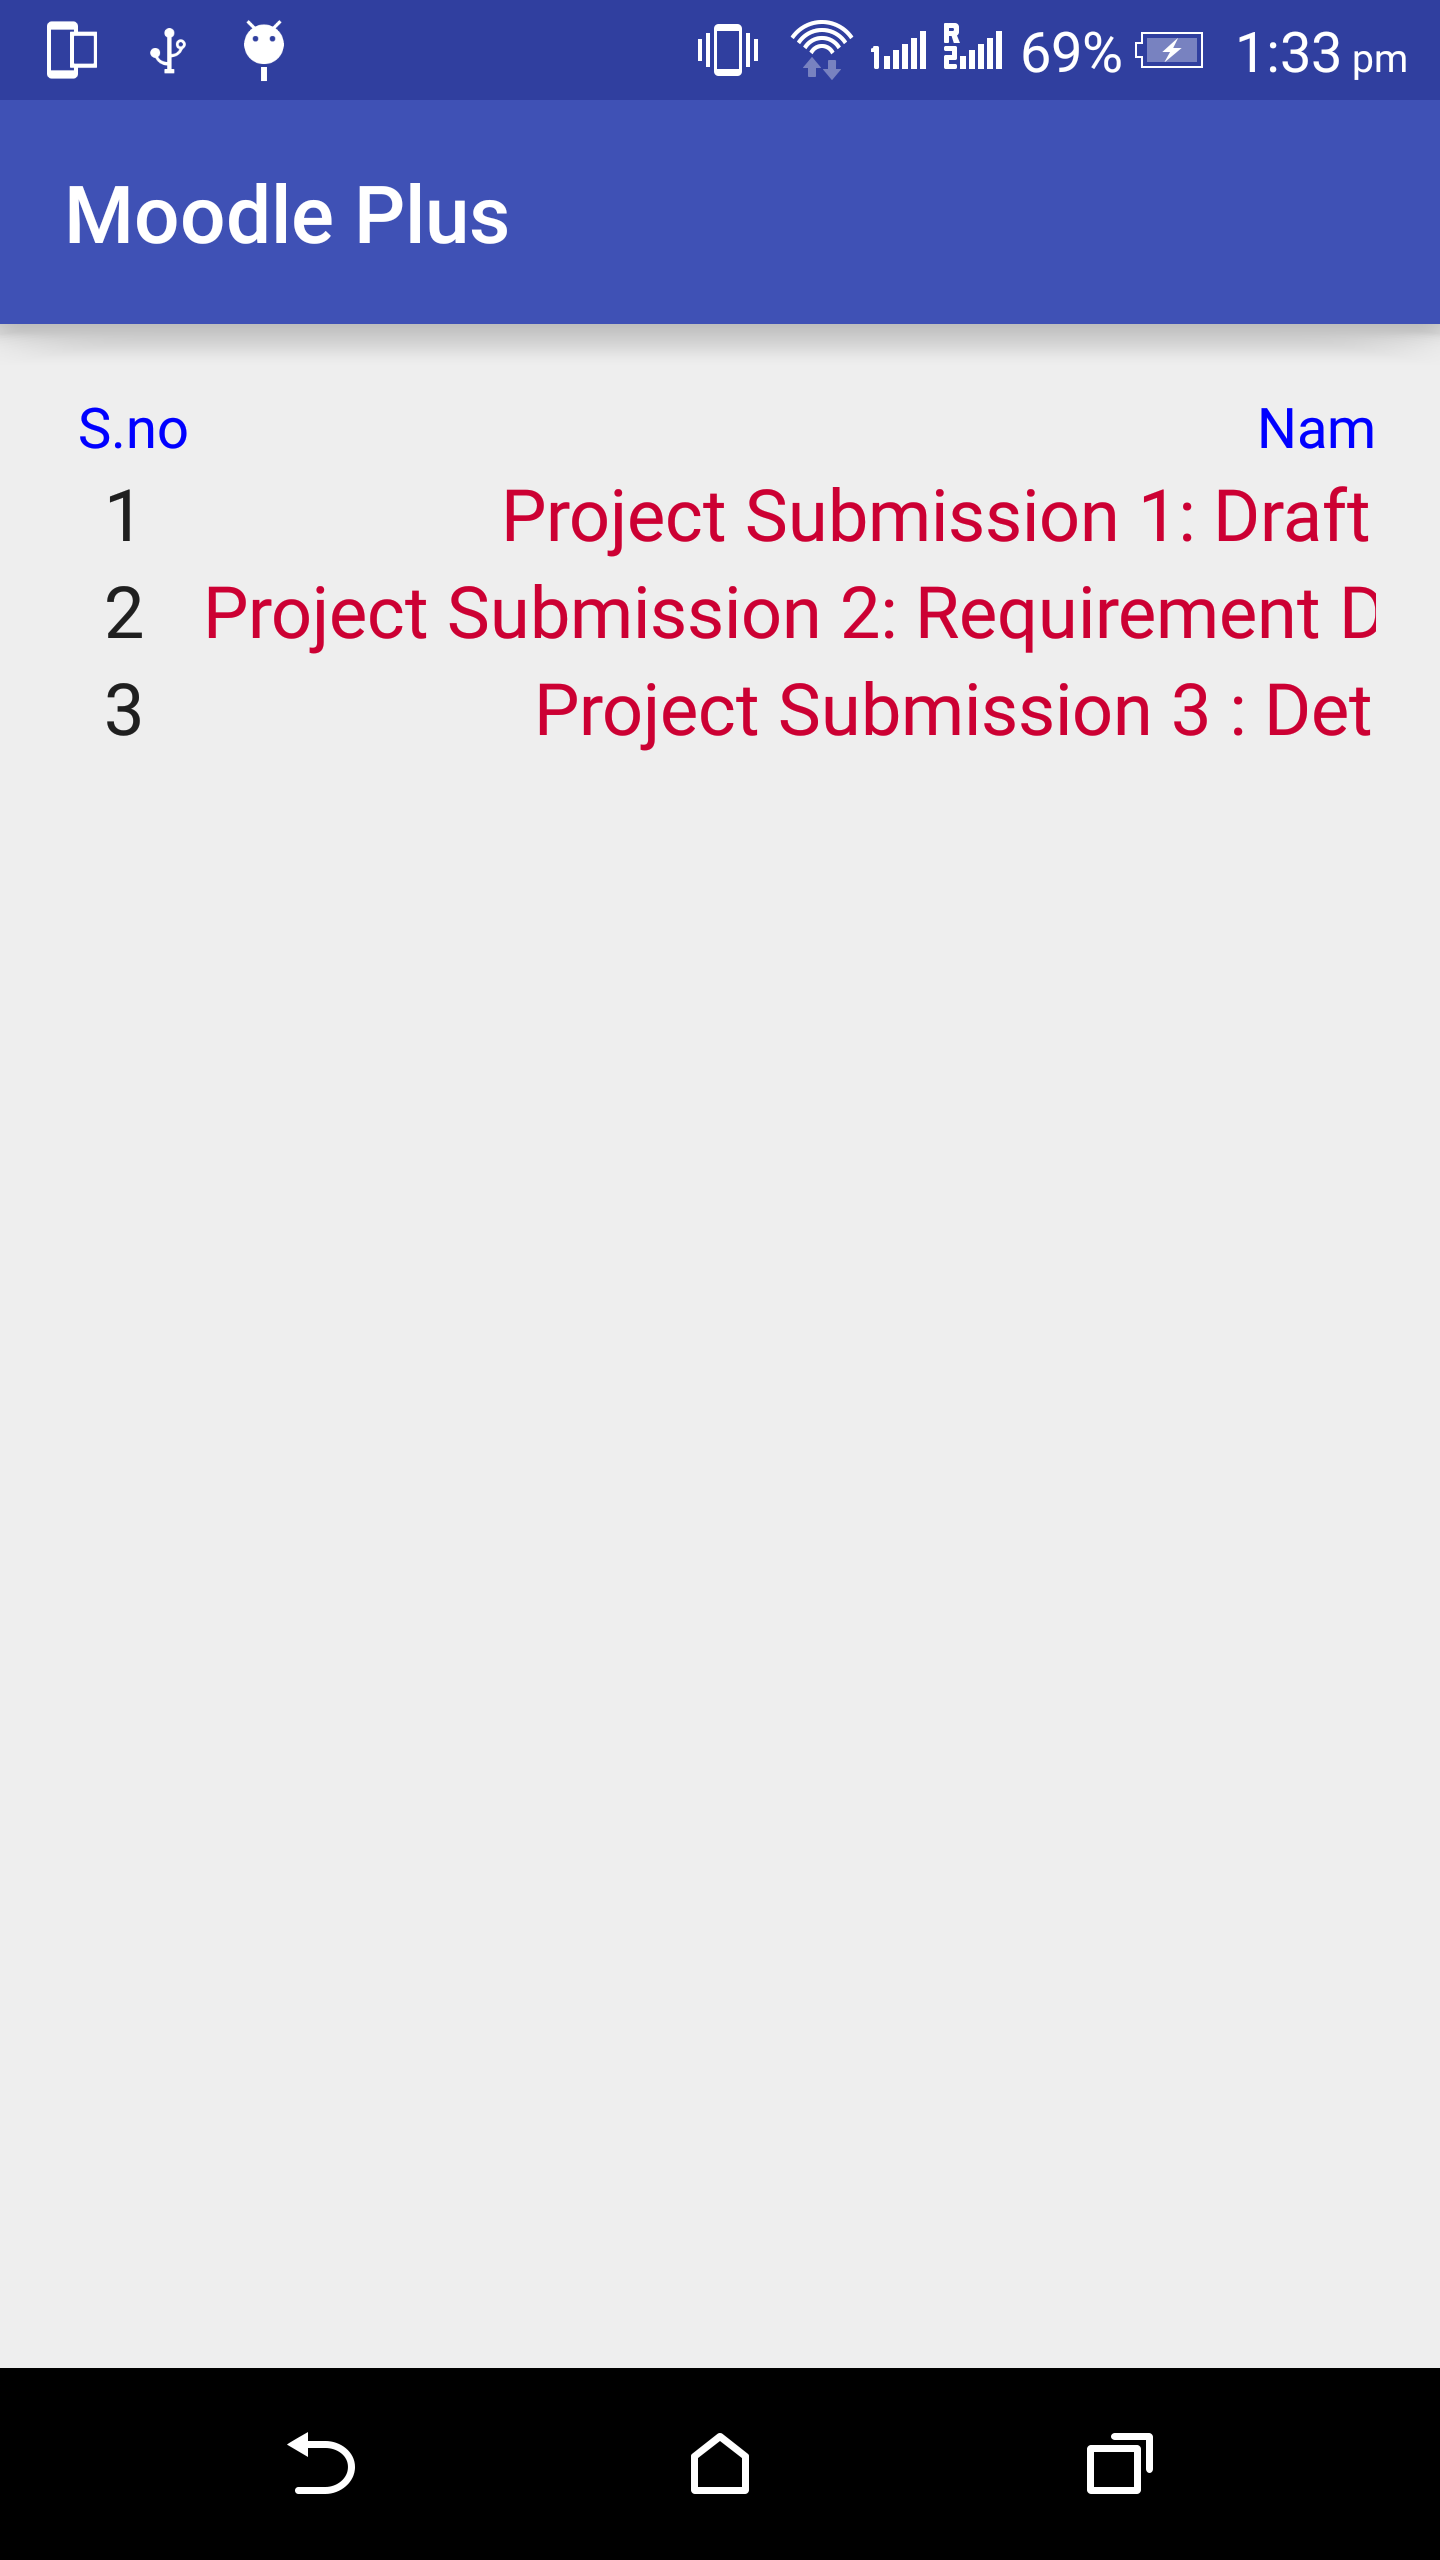
\includegraphics[width=0.4\textwidth]{images/assignments.png}
	\caption{Assignments Screen}
\end{figure}
\FloatBarrier
\subsubsection{Assignment Information}
\begin{figure}[!ht]
	\centering
	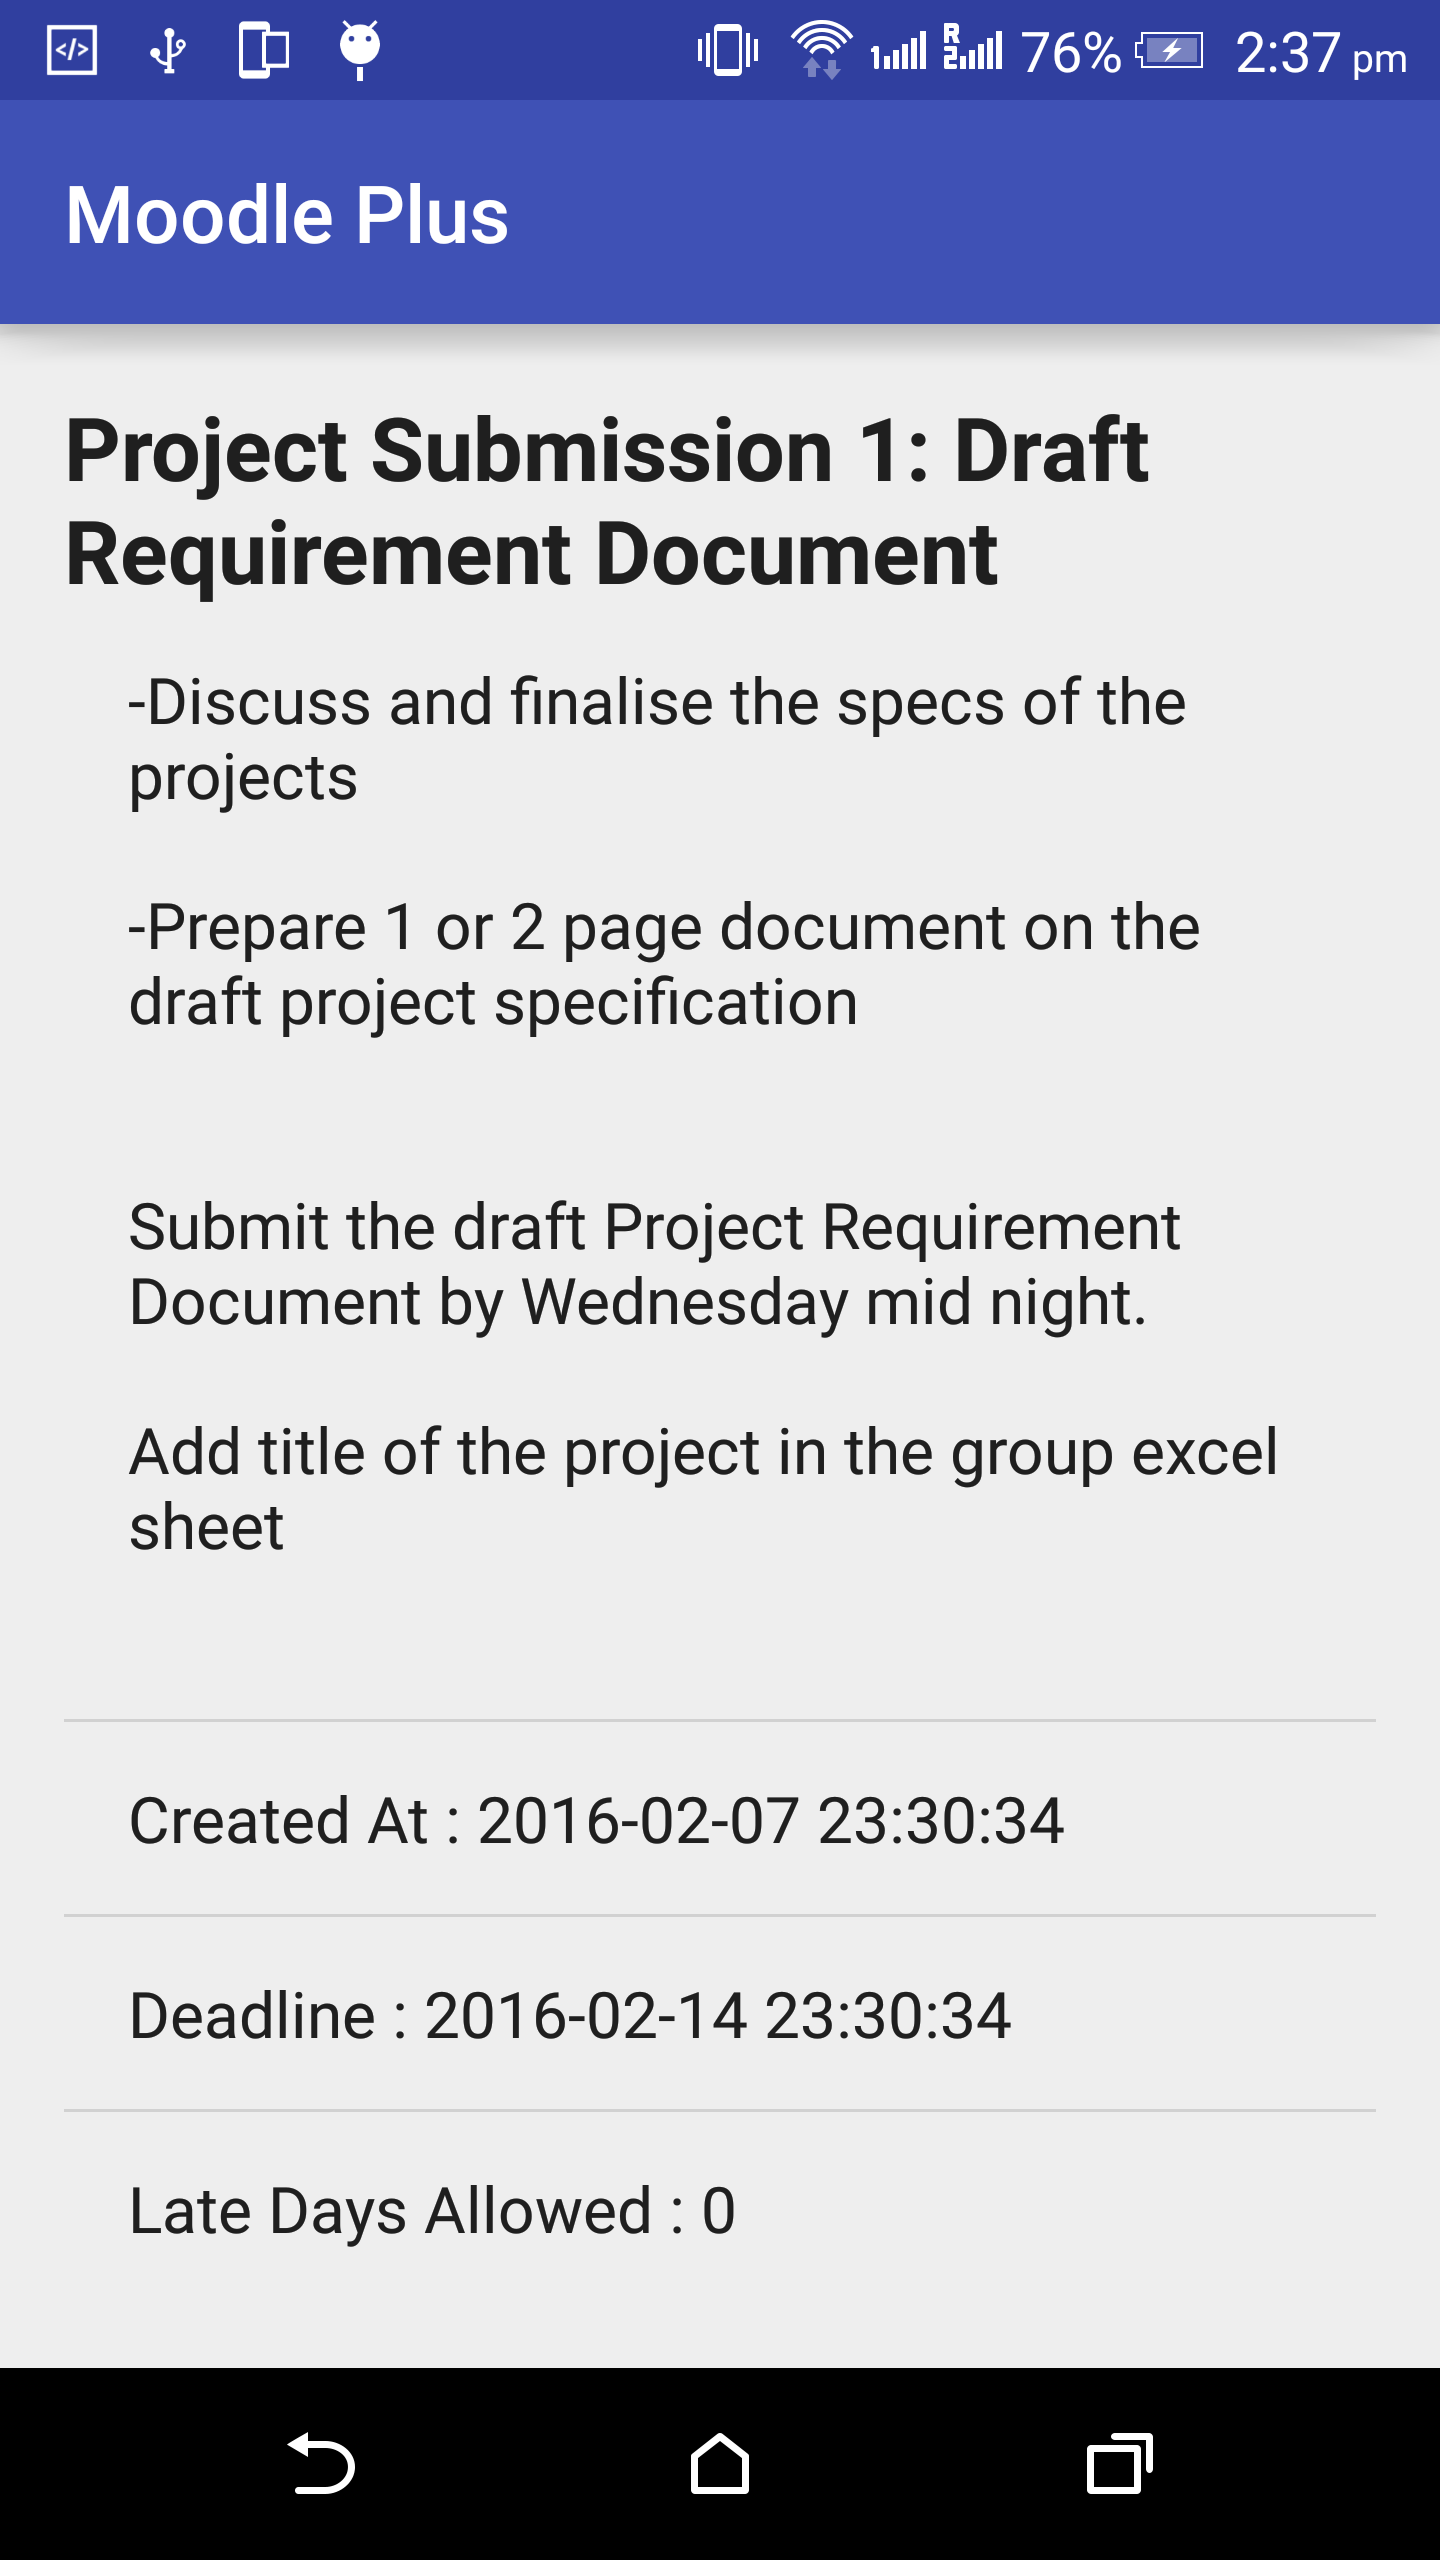
\includegraphics[width=0.4\textwidth]{images/ass_info.png}
	\caption{Assignment Information}
\end{figure}
\FloatBarrier
\subsubsection{Grades}
\begin{figure}[!ht]
	\centering
	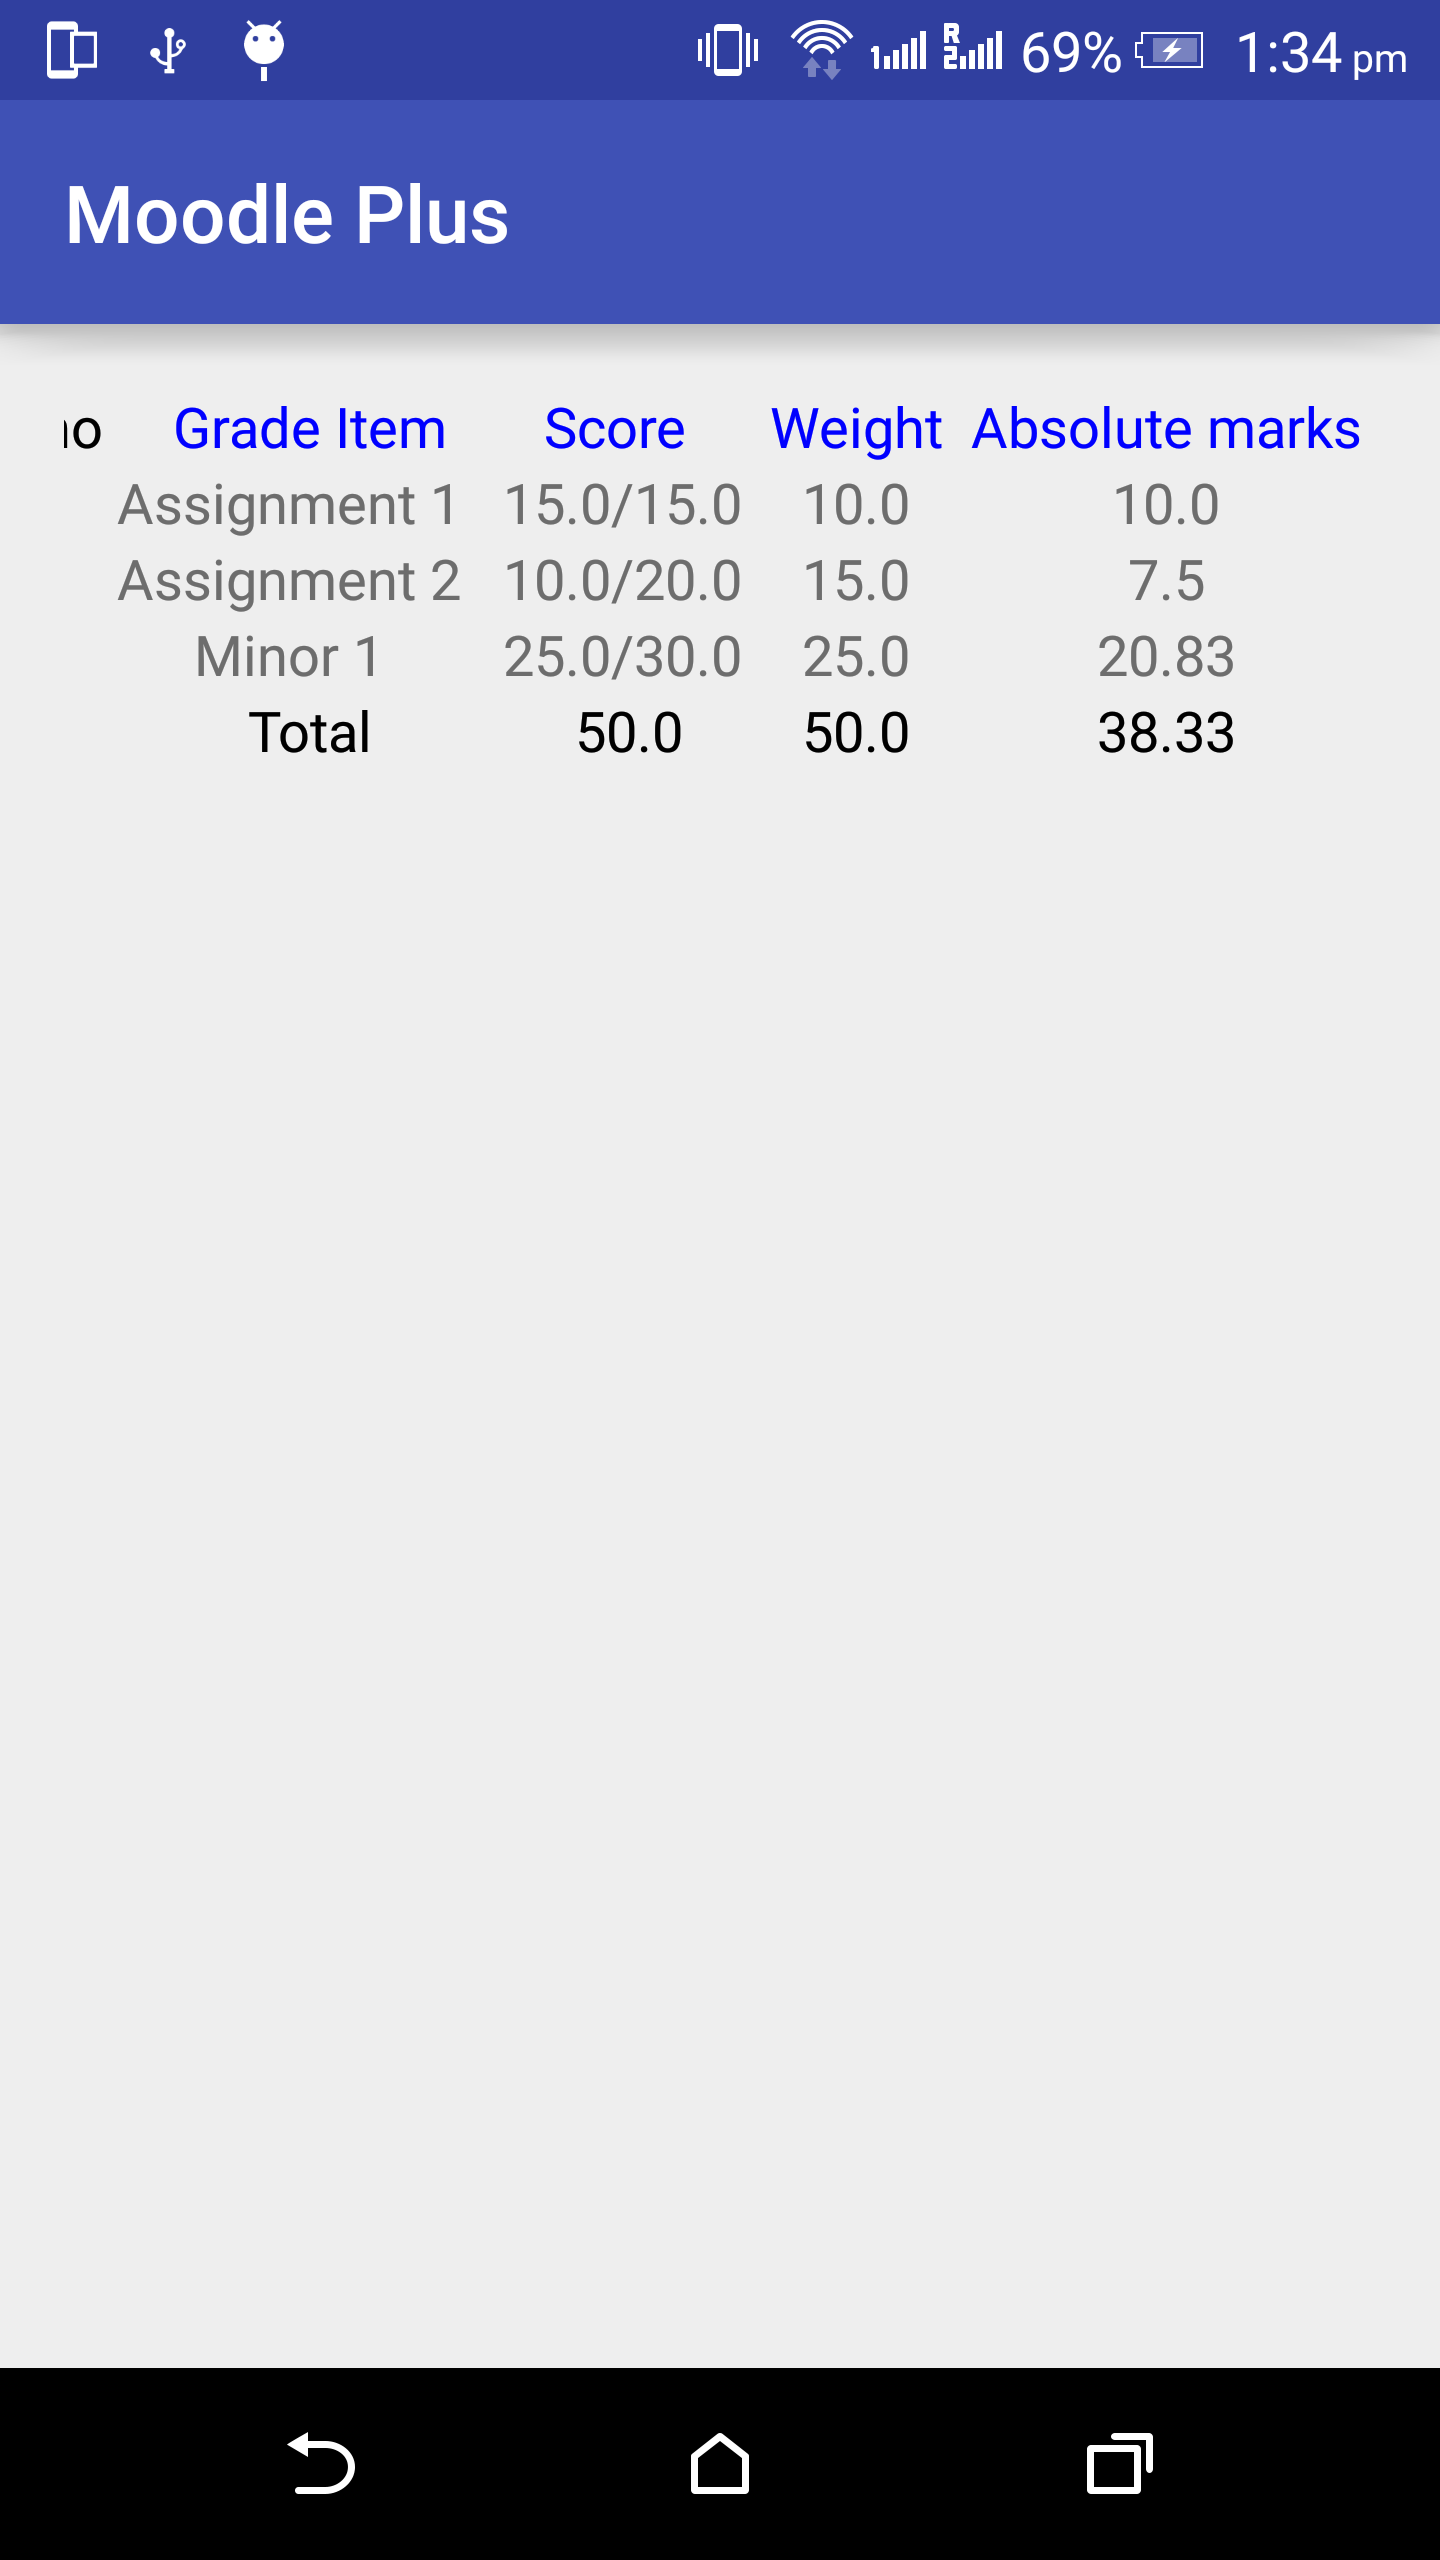
\includegraphics[width=0.4\textwidth]{images/course_grades.png}
	\caption{Grades of the course}
\end{figure}
\FloatBarrier

\subsubsection{List of Threads}
\begin{figure}[!ht]
	\centering
	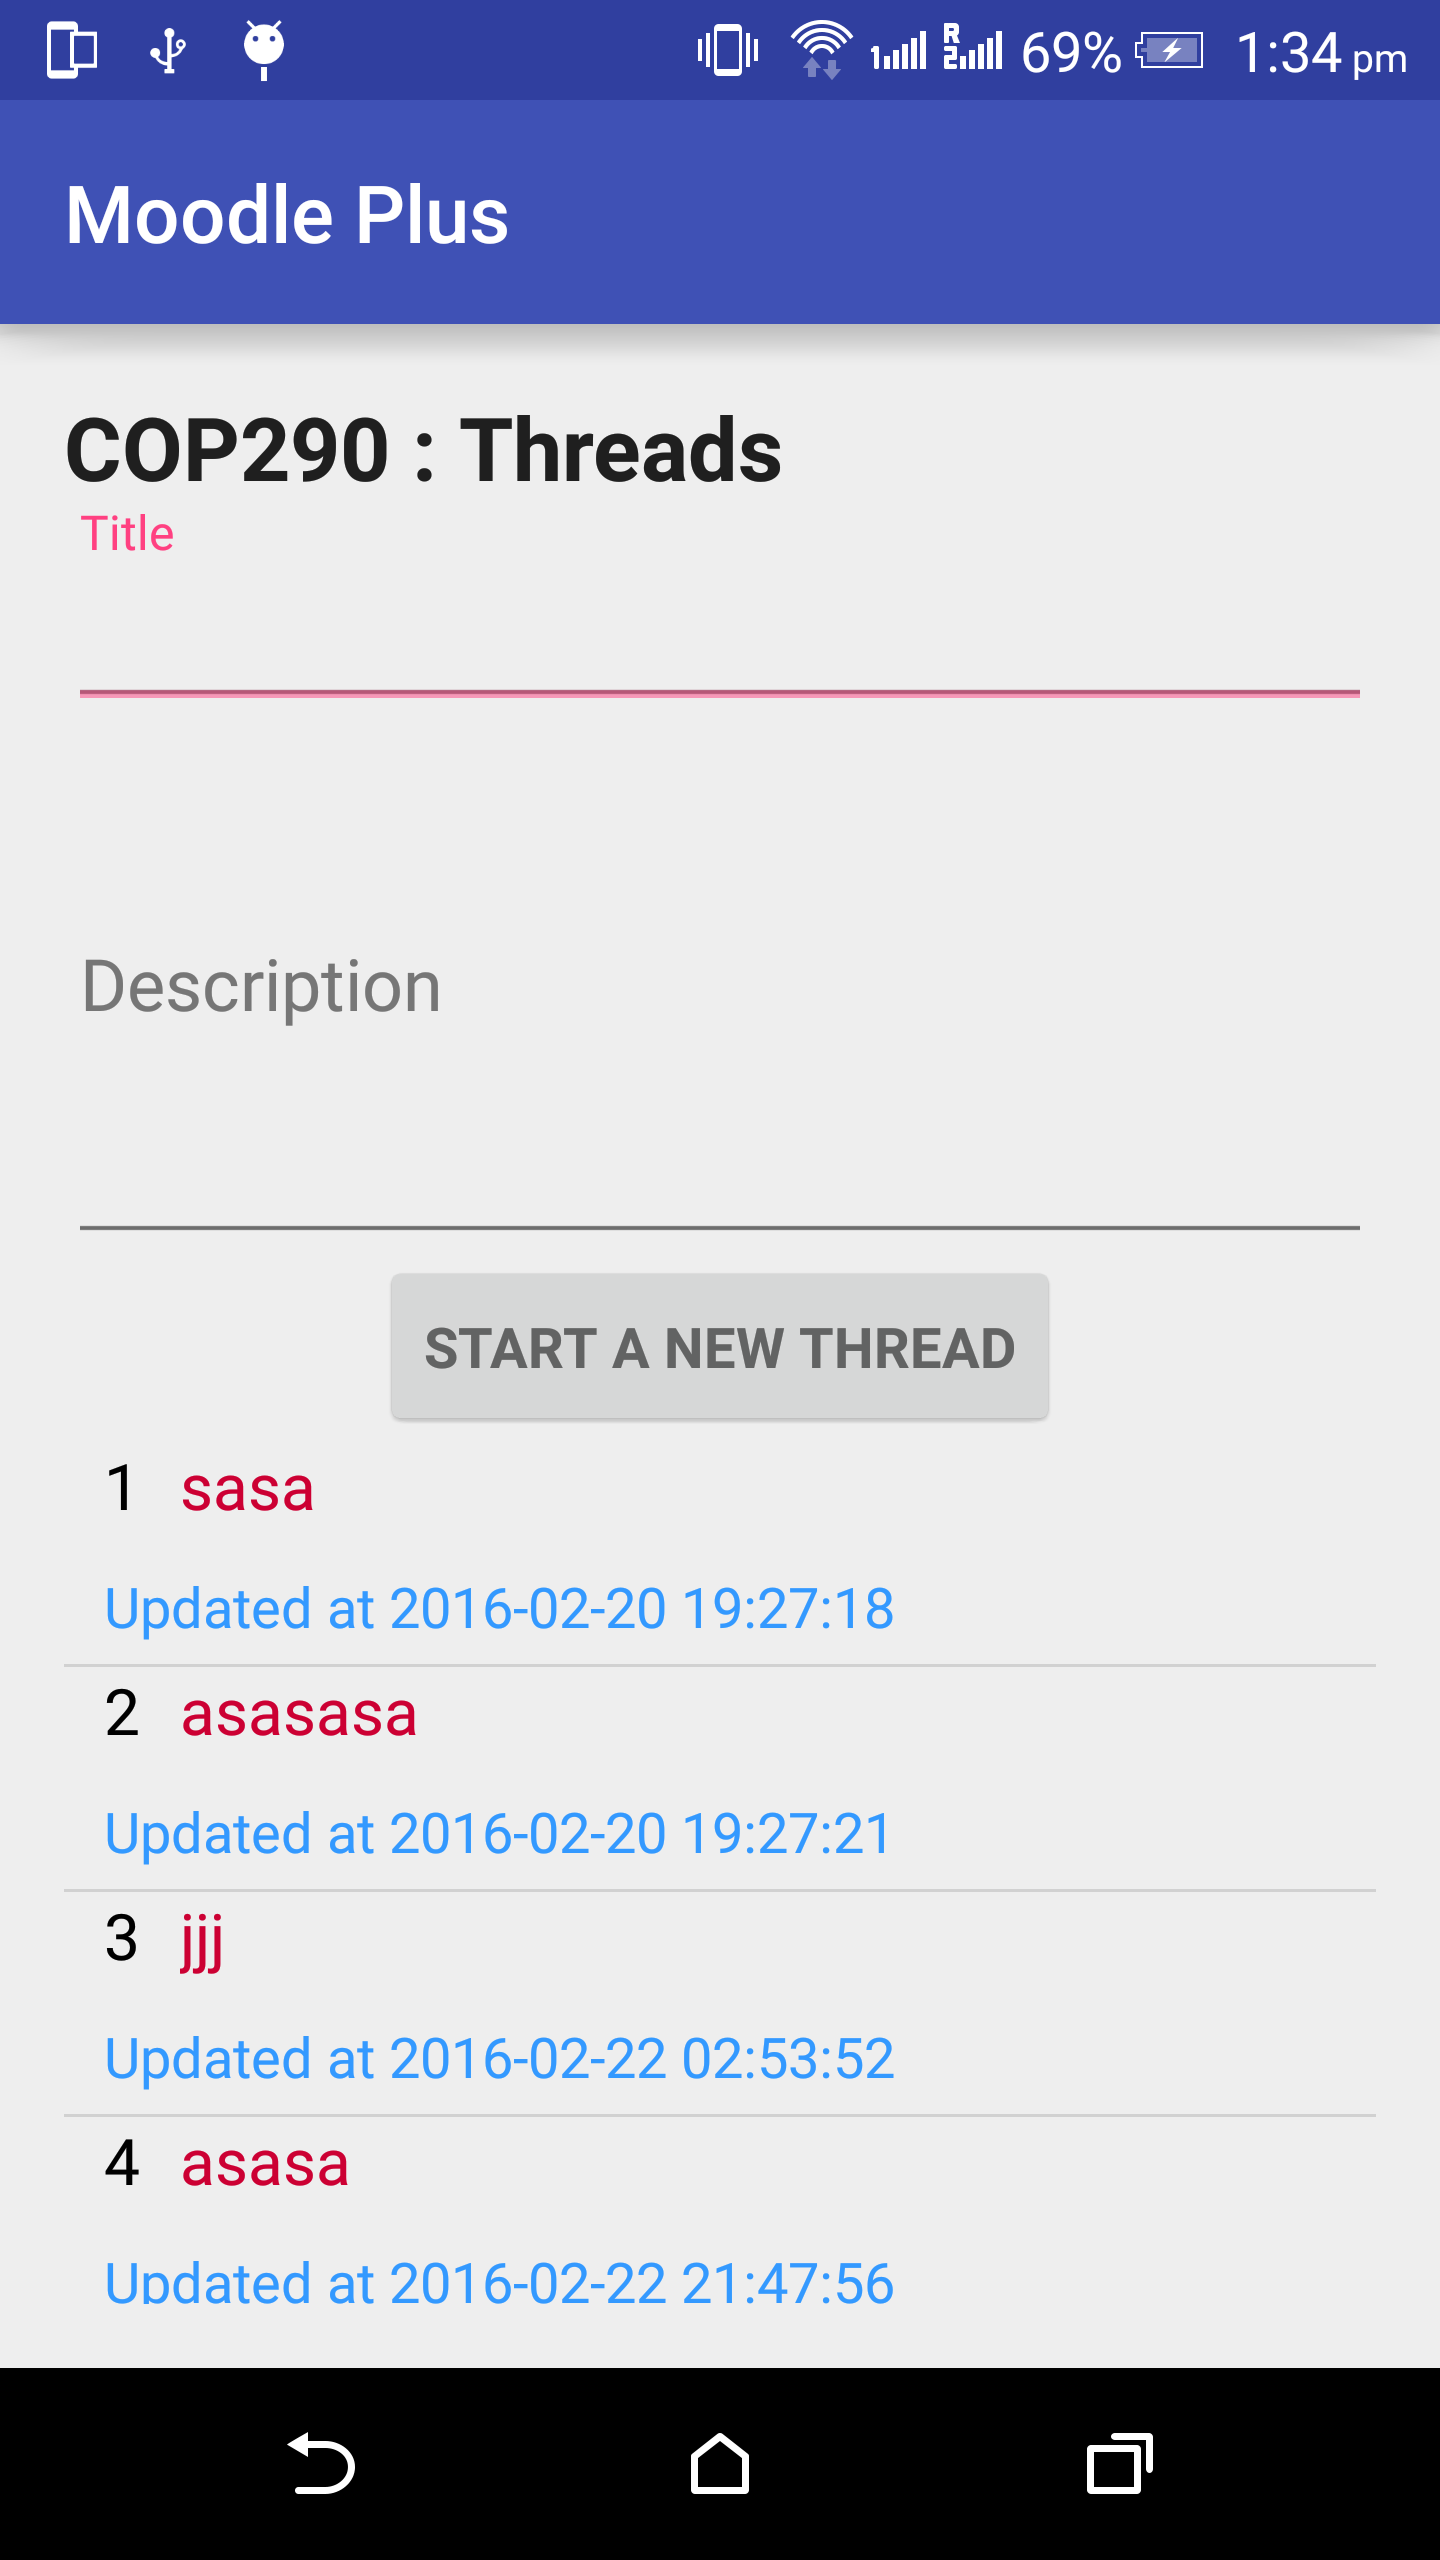
\includegraphics[width=0.4\textwidth]{images/threads.png}
	\caption{Threads}
\end{figure}
\FloatBarrier

\subsubsection{Thread Information and Comments}
\begin{figure}[!ht]
	\centering
	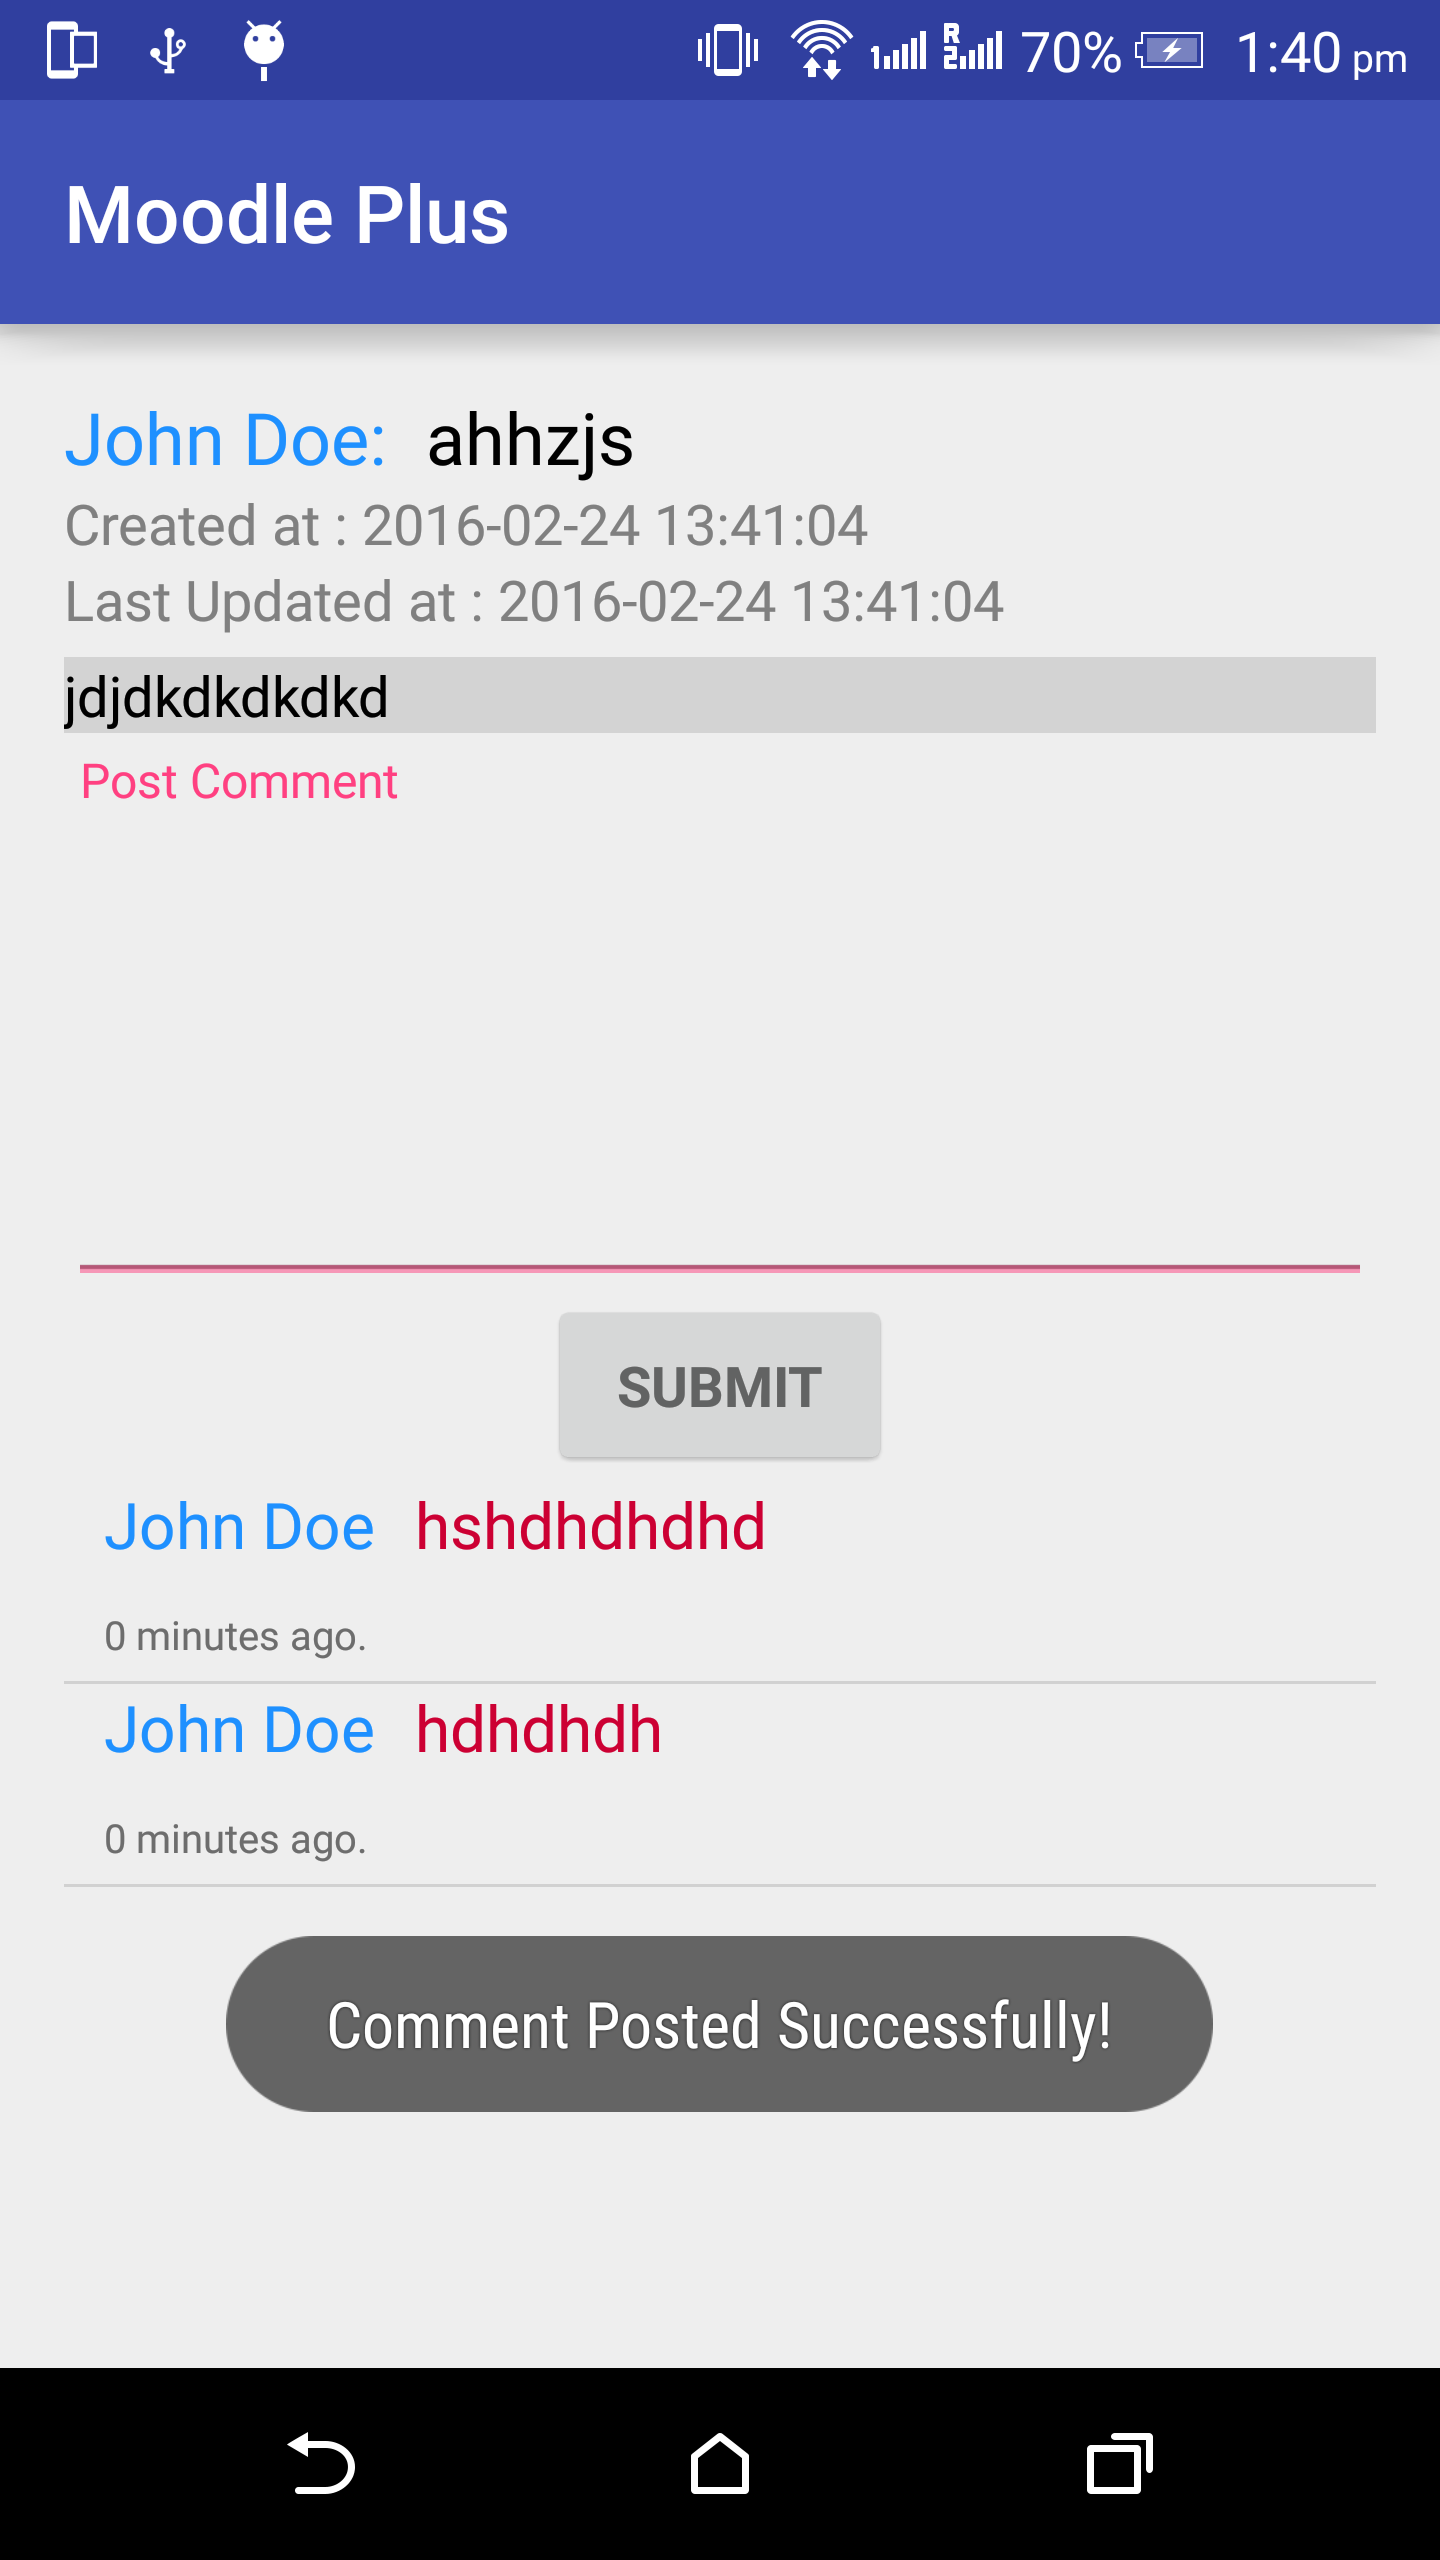
\includegraphics[width=0.4\textwidth]{images/comments.png}
	\caption{Thread Info}
\end{figure}
\FloatBarrier
\section{Implementation Details}
\subsection{Classes}
The following classes were created for storing and handling necessary information from the HTTP GET response.
All the classes below implement \textbf{Parcelable}\cite{parcel} interface to pass data from one activity to another activity.
\subsubsection{User}
\subsubsection{Course}
\subsubsection{AssignmentInfo}
\subsubsection{Grades}
\subsubsection{Thread}
\subsubsection{Thread\_Comments}
\subsubsection{Notification}

\subsection{Activities}

\subsubsection{LoginActivity}
The initial activity of the application where the user is expected to login his credentials.If the credentials are incorrect, a toast message is displayed conveying the same. On successful login , the JSON response from the server is parsed and the necessary information is stored in an object of \textbf{User} class and this information is passed to the next activity (\textbf{CoursesList}). 
\subsubsection{CoursesList}
This activity corresponds to the Welcome or Home screen where all the registered courses are listed.On clicking any particular course, it redirects to CourseContent activity.
\subsubsection{CourseContent}
This activity is for displaying  various contents of the course like Assignments,Grades \& Threads.
\subsubsection{CourseGrades}
This activity is for displaying the grades of a particular course.
\subsubsection{ListofAssignmnets}
This activity is for displaying the list of assignments of a particular course.
\subsubsection{AssignmentInfo}
This activity is for displaying the information of a particular assignment like description,late days available,deadline etc.
\subsubsection{ThreadsList}
Facilitates posting of new threads apart from displaying the list of threads.
\subsubsection{ThreadInfo}
Facilitates posting of comments to any particular thread apart from displaying the information of the current thread.
\subsubsection{GradesAll}
For displaying grades of all registered courses in one screen.
\subsubsection{Notifications}

\subsection{Methods for network communication}
In this assignment, we used Android provided \textbf{HttpURLConnection} and \textbf{URL}					
classes to handle HTTP GET requests.\cite{Volley}.

\subsubsection{Cookie Handling}

We used Android provided \textbf{CookieHandler,CookieManager}  classes to manage cookies. 
\section{VCS}
The code for the project is being maintained in this repository:\\
\textbf{{\em     https://saideepbsd@bitbucket.org/saideepbsd/a1.git}}

\bibliographystyle{abbrv}
\bibliography{references}

\end{document}
